\section{Messergebnisse und Auswertung}

\subsection{Vorgehensweise bei der Auswertung}
Fehler: immer ein Bin.\\
Beispiel: R1
\begin{figure}[H]
\begin{center}
  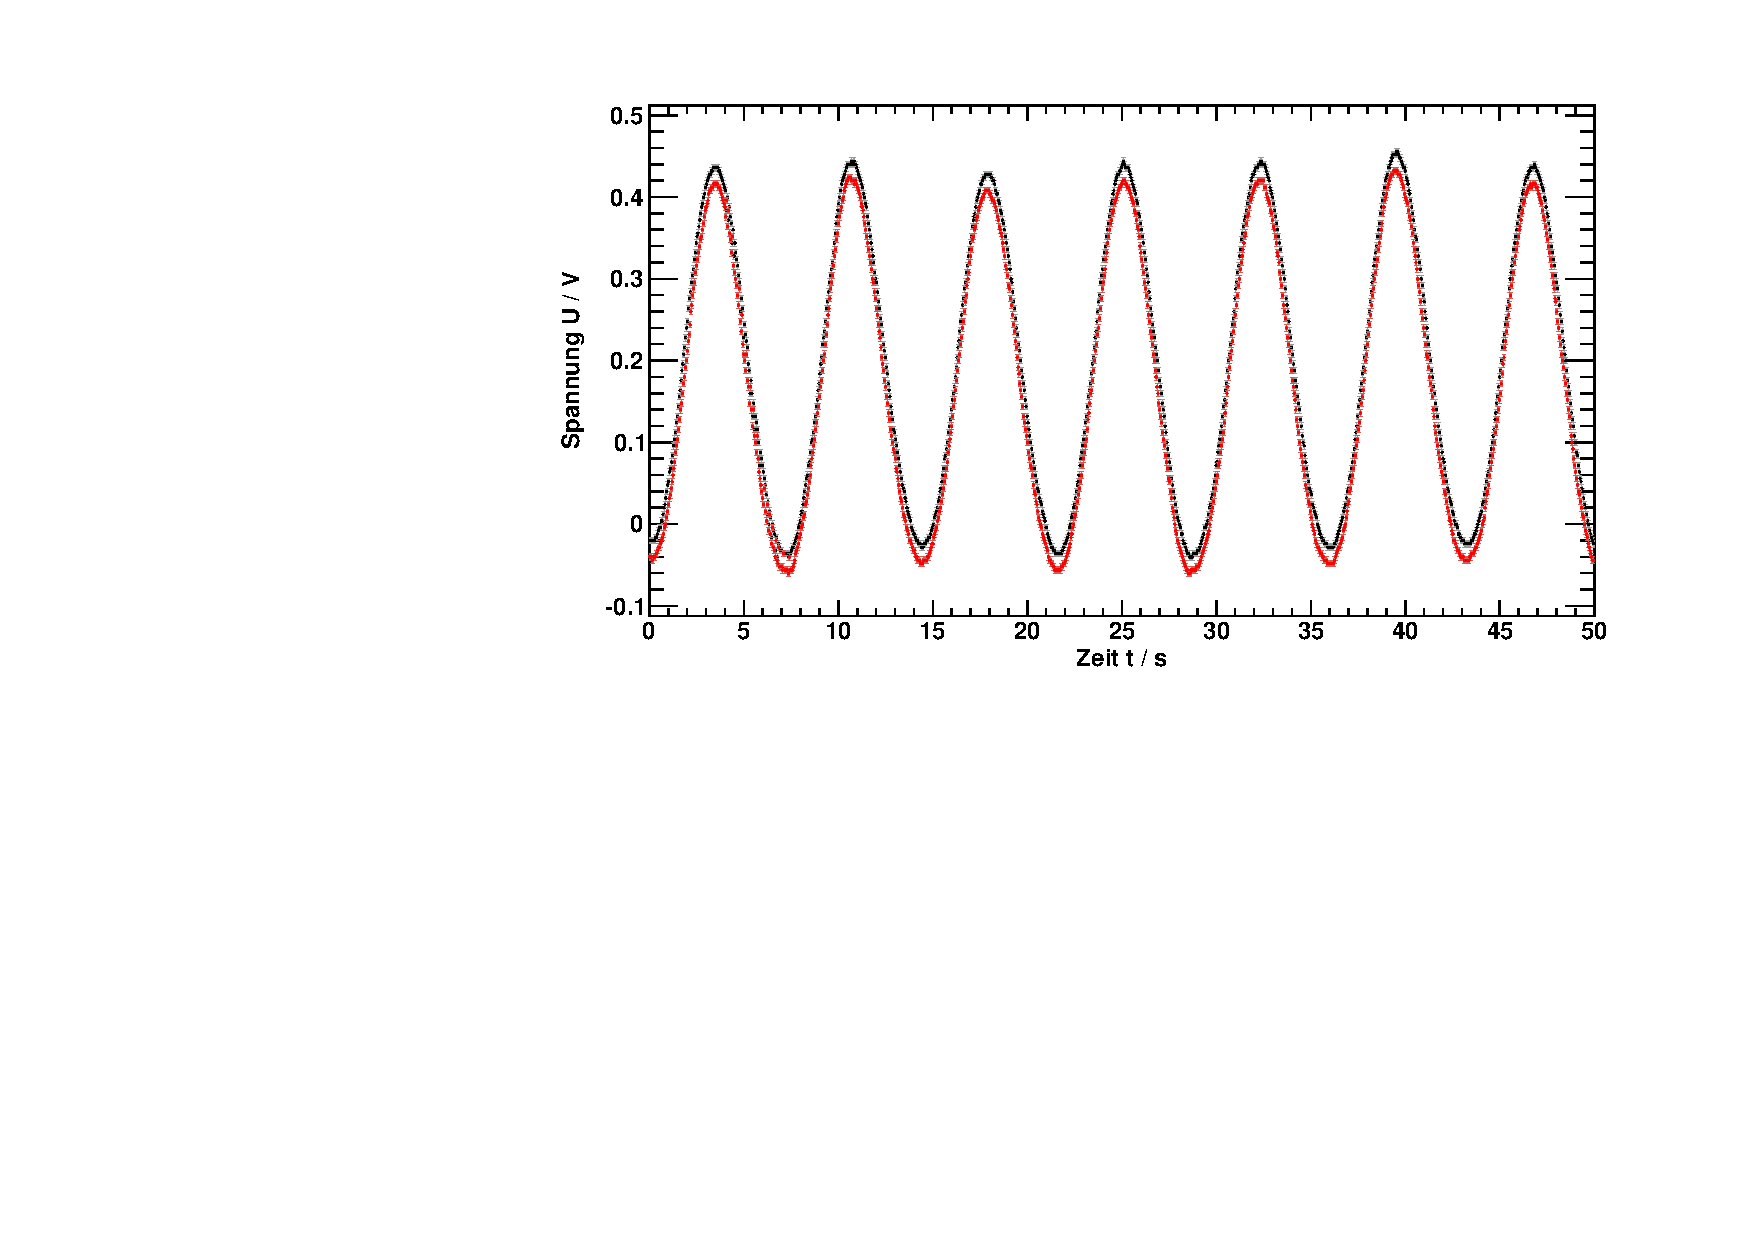
\includegraphics[width=\textwidth]{../img/both_Spule_R1.pdf}
  \caption{caption}
  \label{img:ex:both}
\end{center}
\end{figure}

\begin{figure}[H]
\begin{center}
  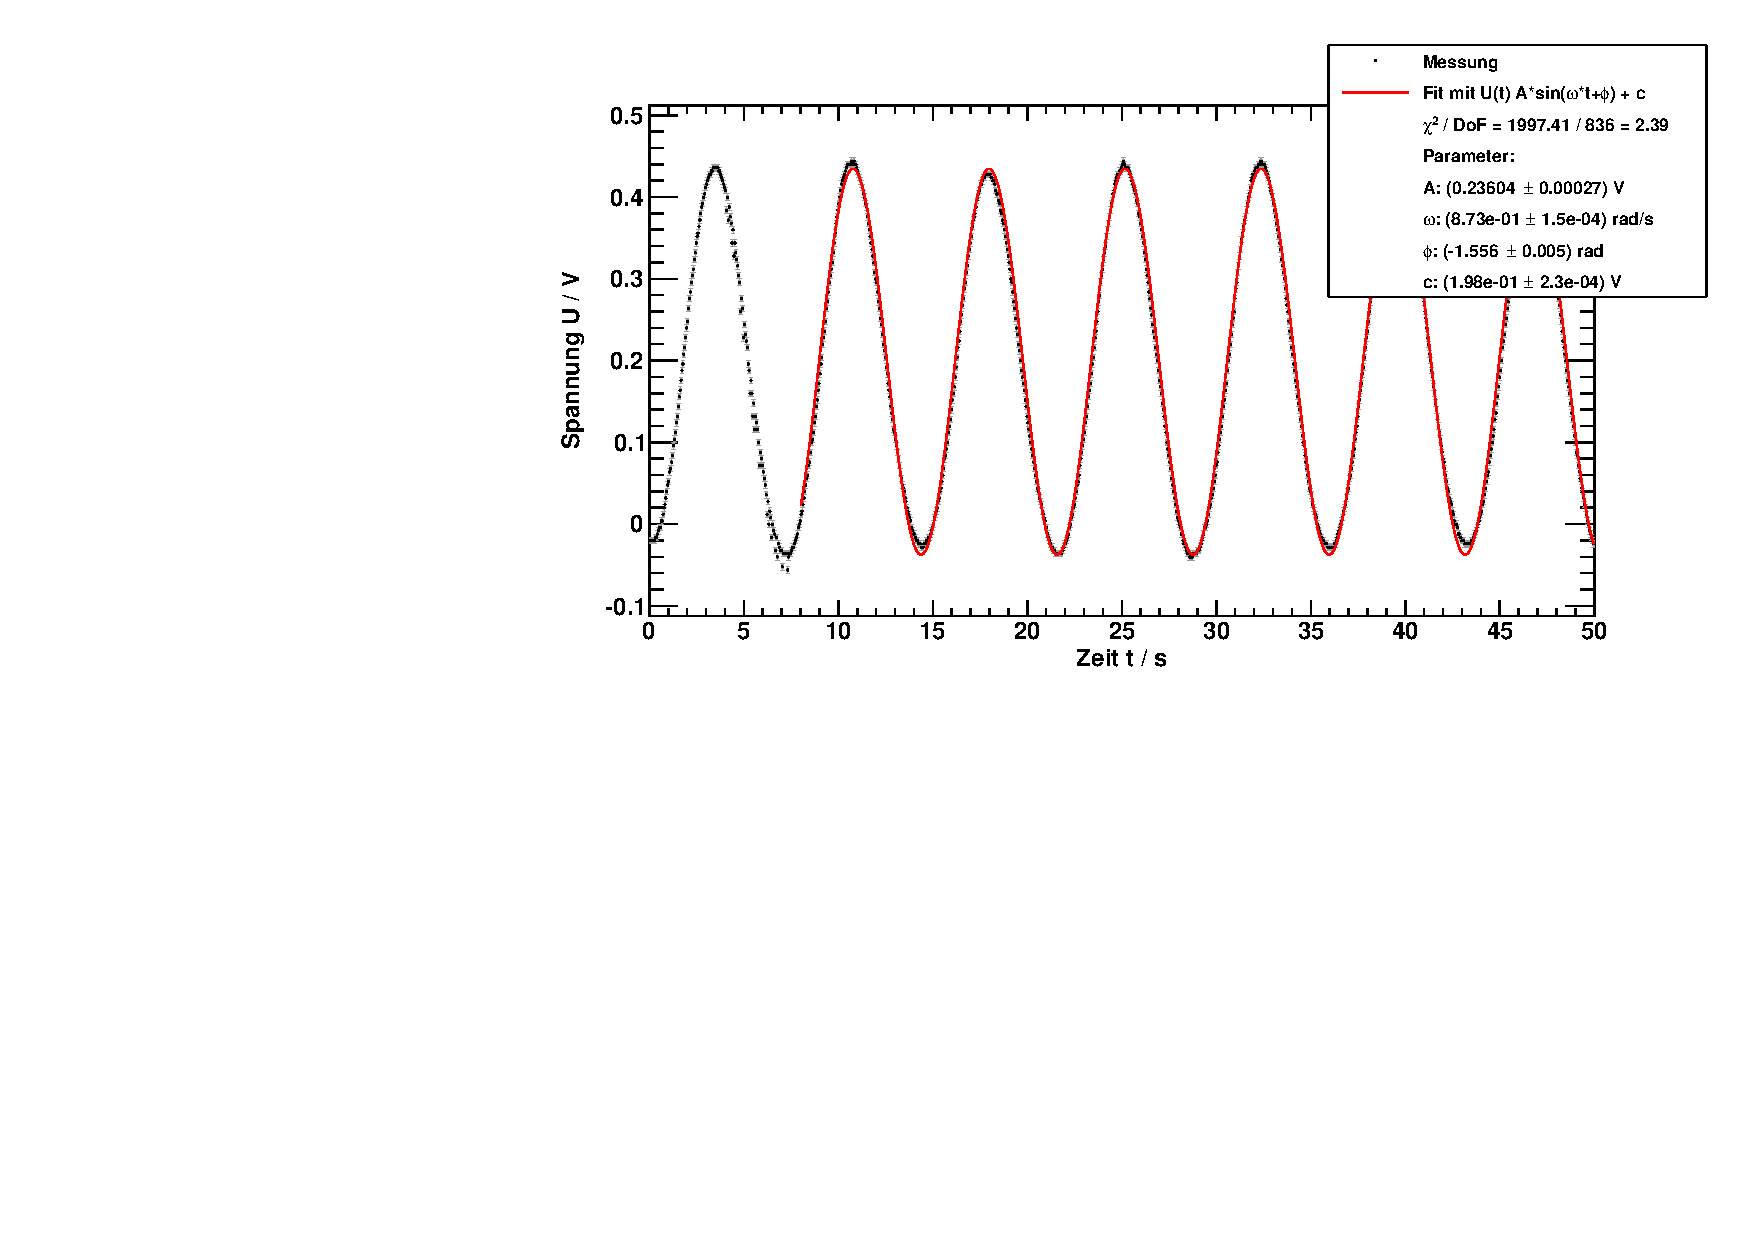
\includegraphics[width=\textwidth]{../img/fit_Spule_R1.pdf}
  \caption{caption}
  \label{img:ex:fit}
\end{center}
\end{figure}
\begin{figure}[H]
\begin{center}
  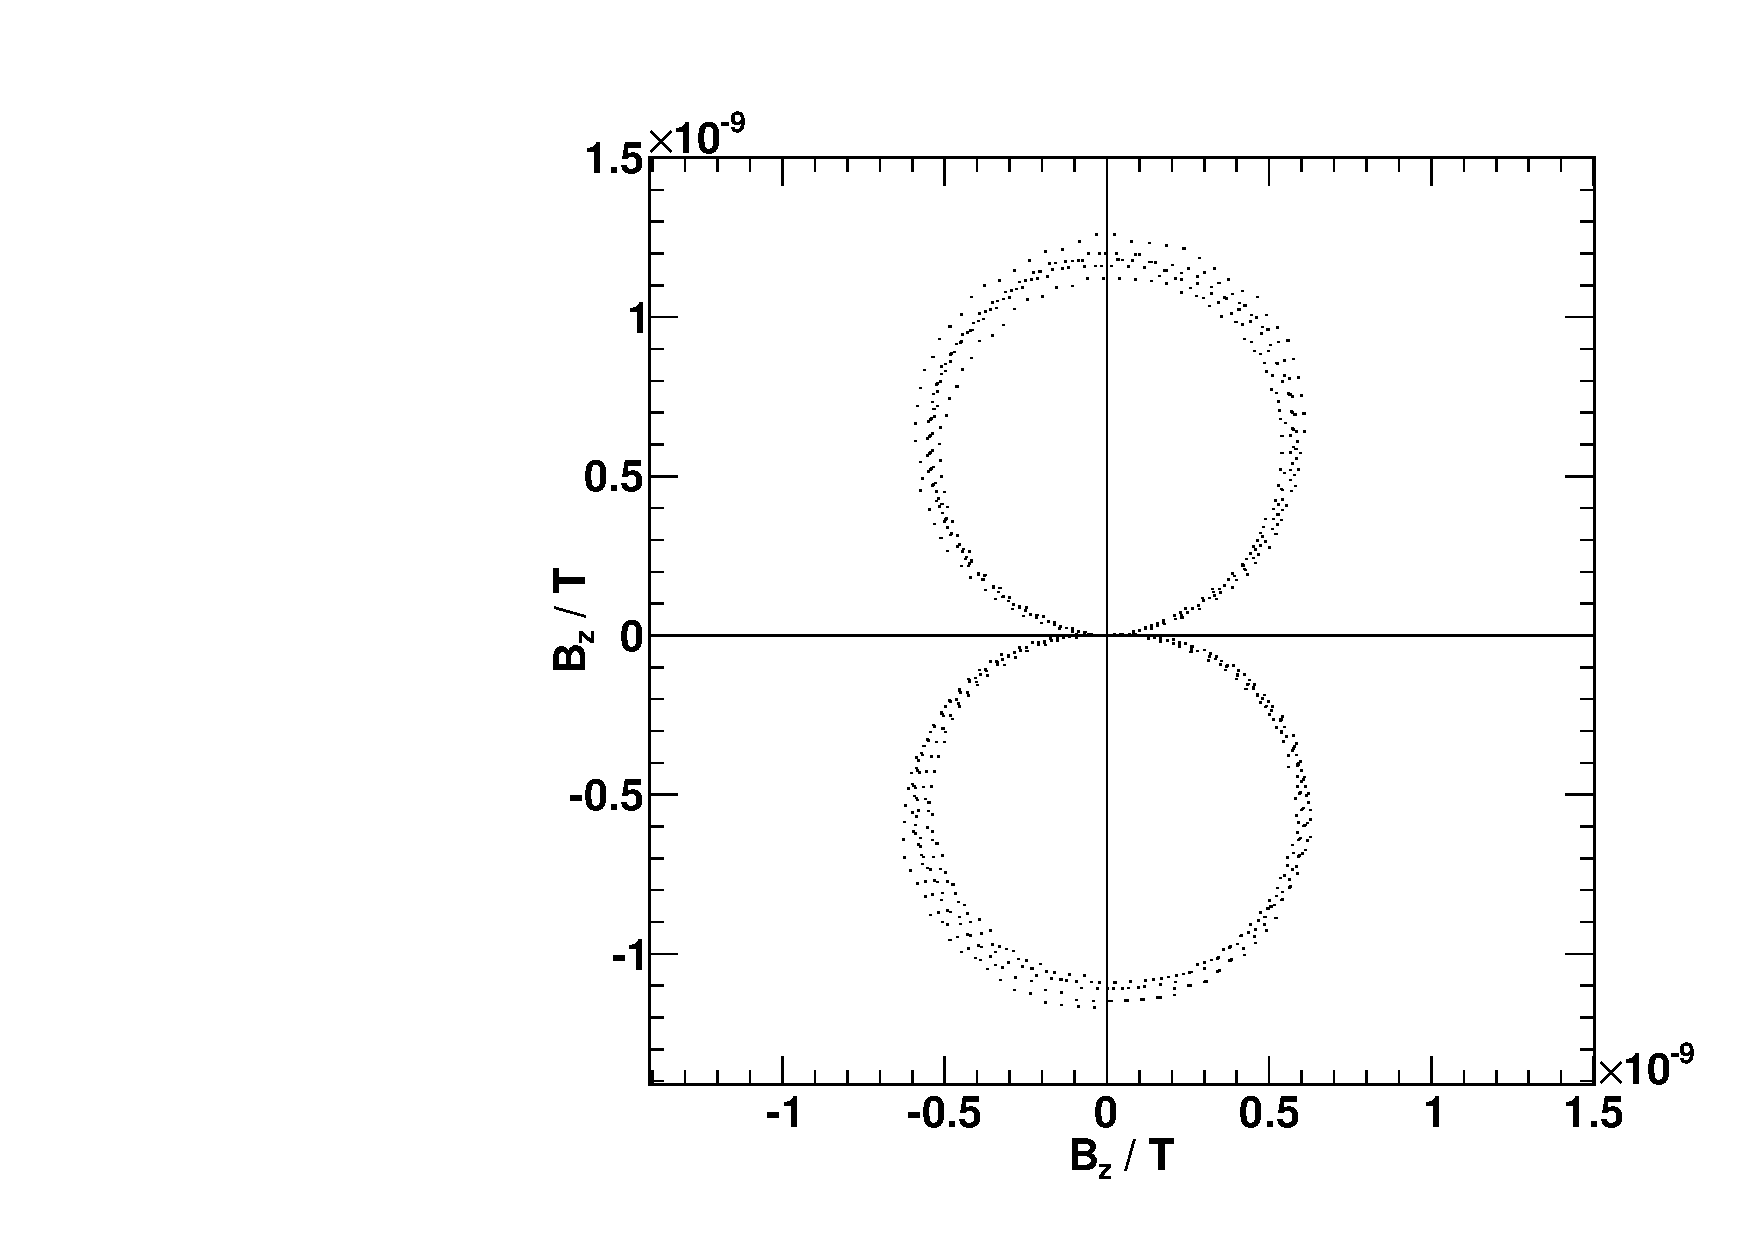
\includegraphics[width=0.5\textwidth]{../img/polar_Spule_R1.pdf}
  \caption{caption}
  \label{img:ex:polar}
\end{center}
\end{figure}

\subsection{Vermessung des Magnetfeldes der Leiterschleife}
\subsubsection{Berechnung aus der SQUID-Messung}
\begin{figure}[H]
\begin{center}
  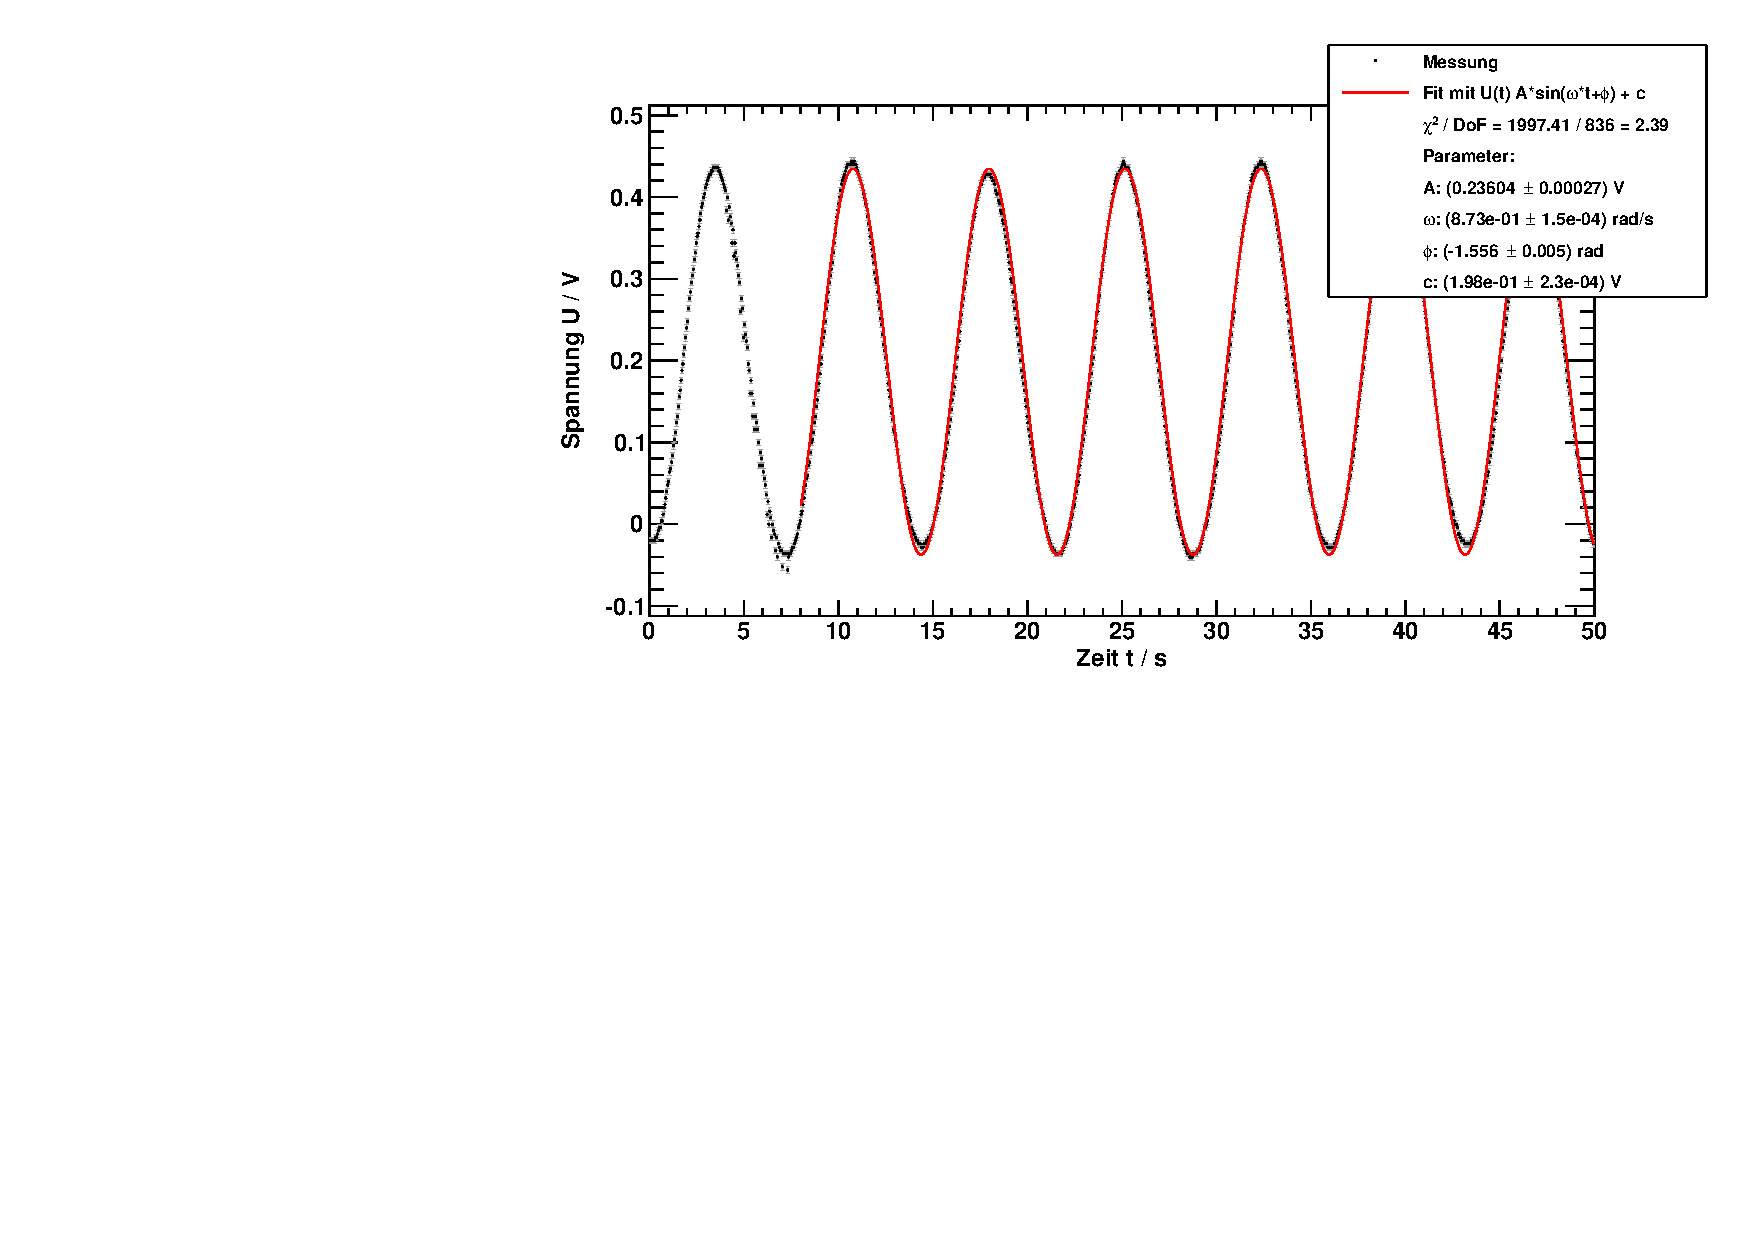
\includegraphics[width=0.64\textwidth]{../img/fit_Spule_R1.pdf}
  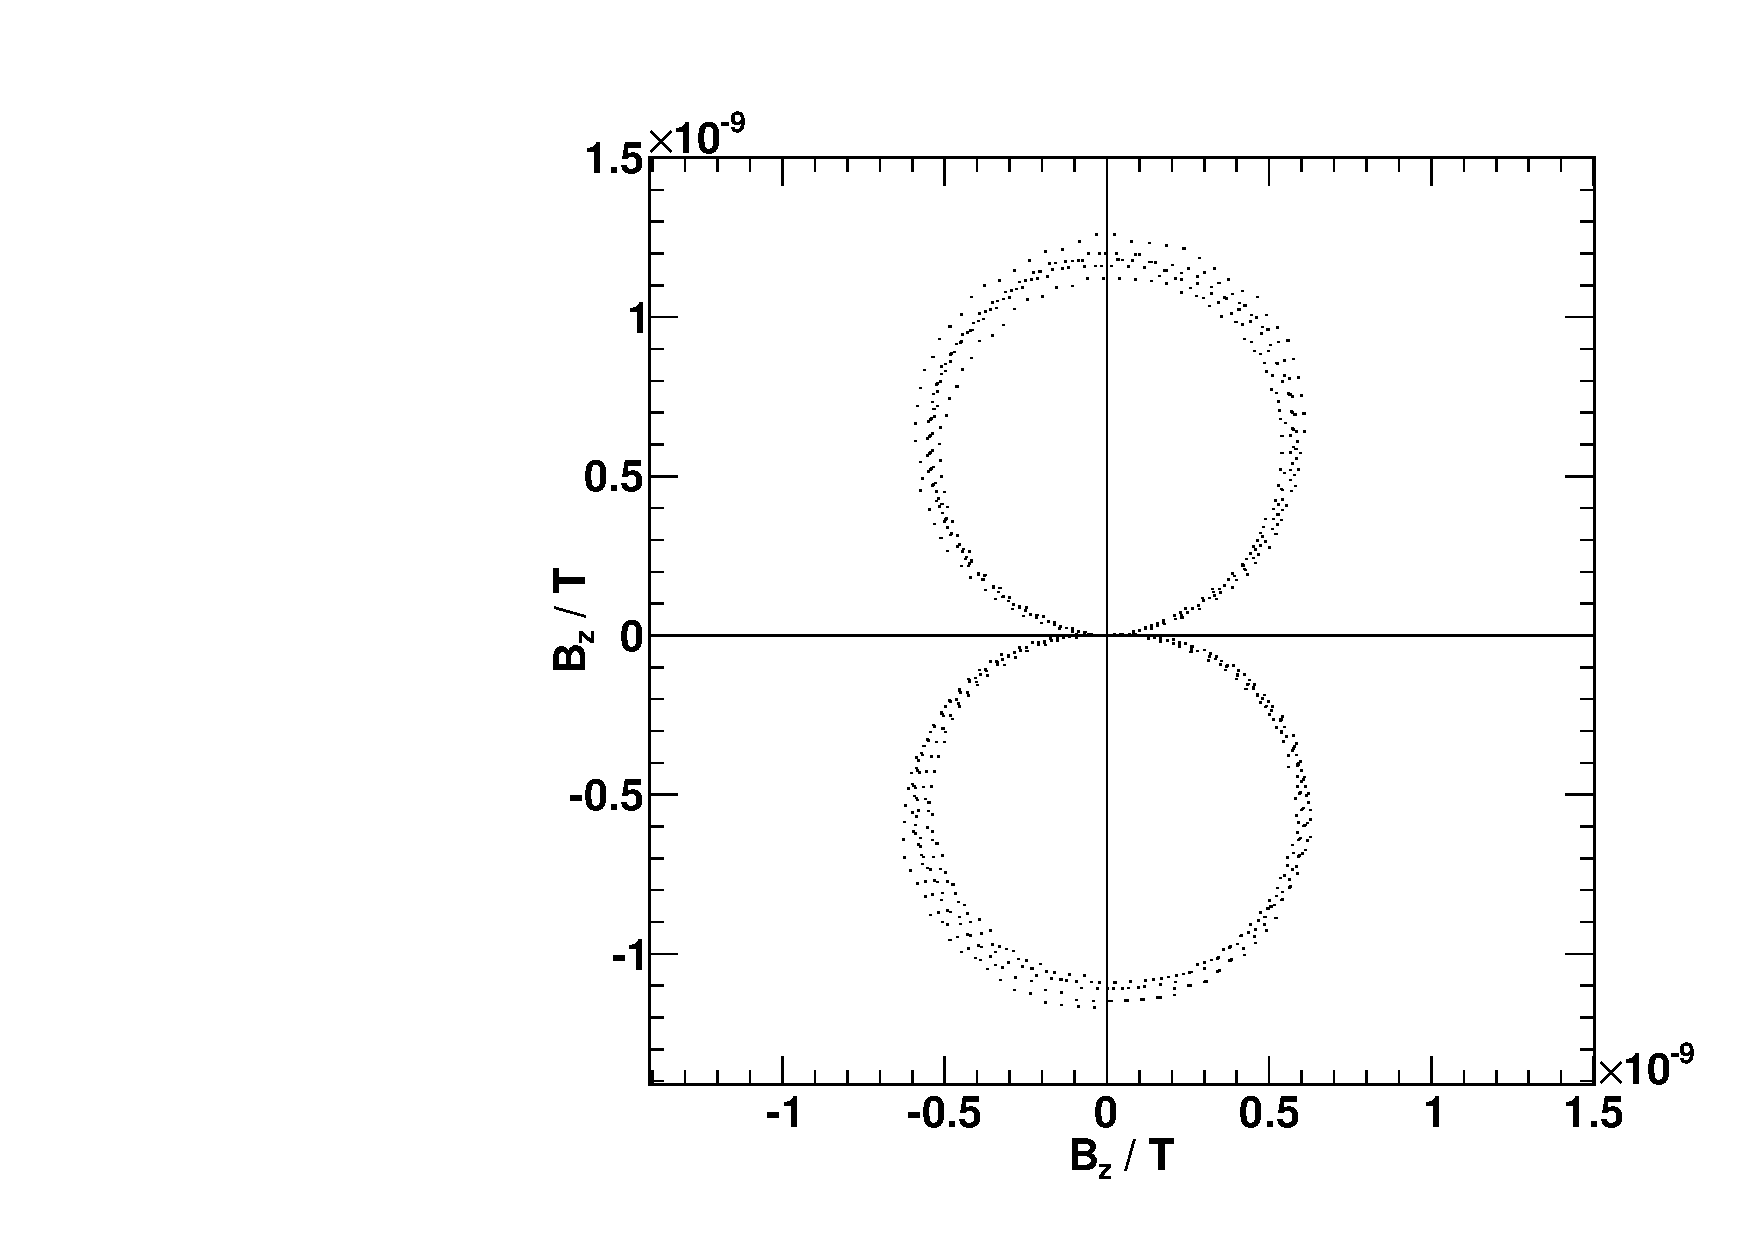
\includegraphics[width=0.35\textwidth]{../img/polar_Spule_R1.pdf}
  \caption{caption}
  \label{img:R1}
\end{center}
\end{figure}

\begin{figure}[H]
\begin{center}
  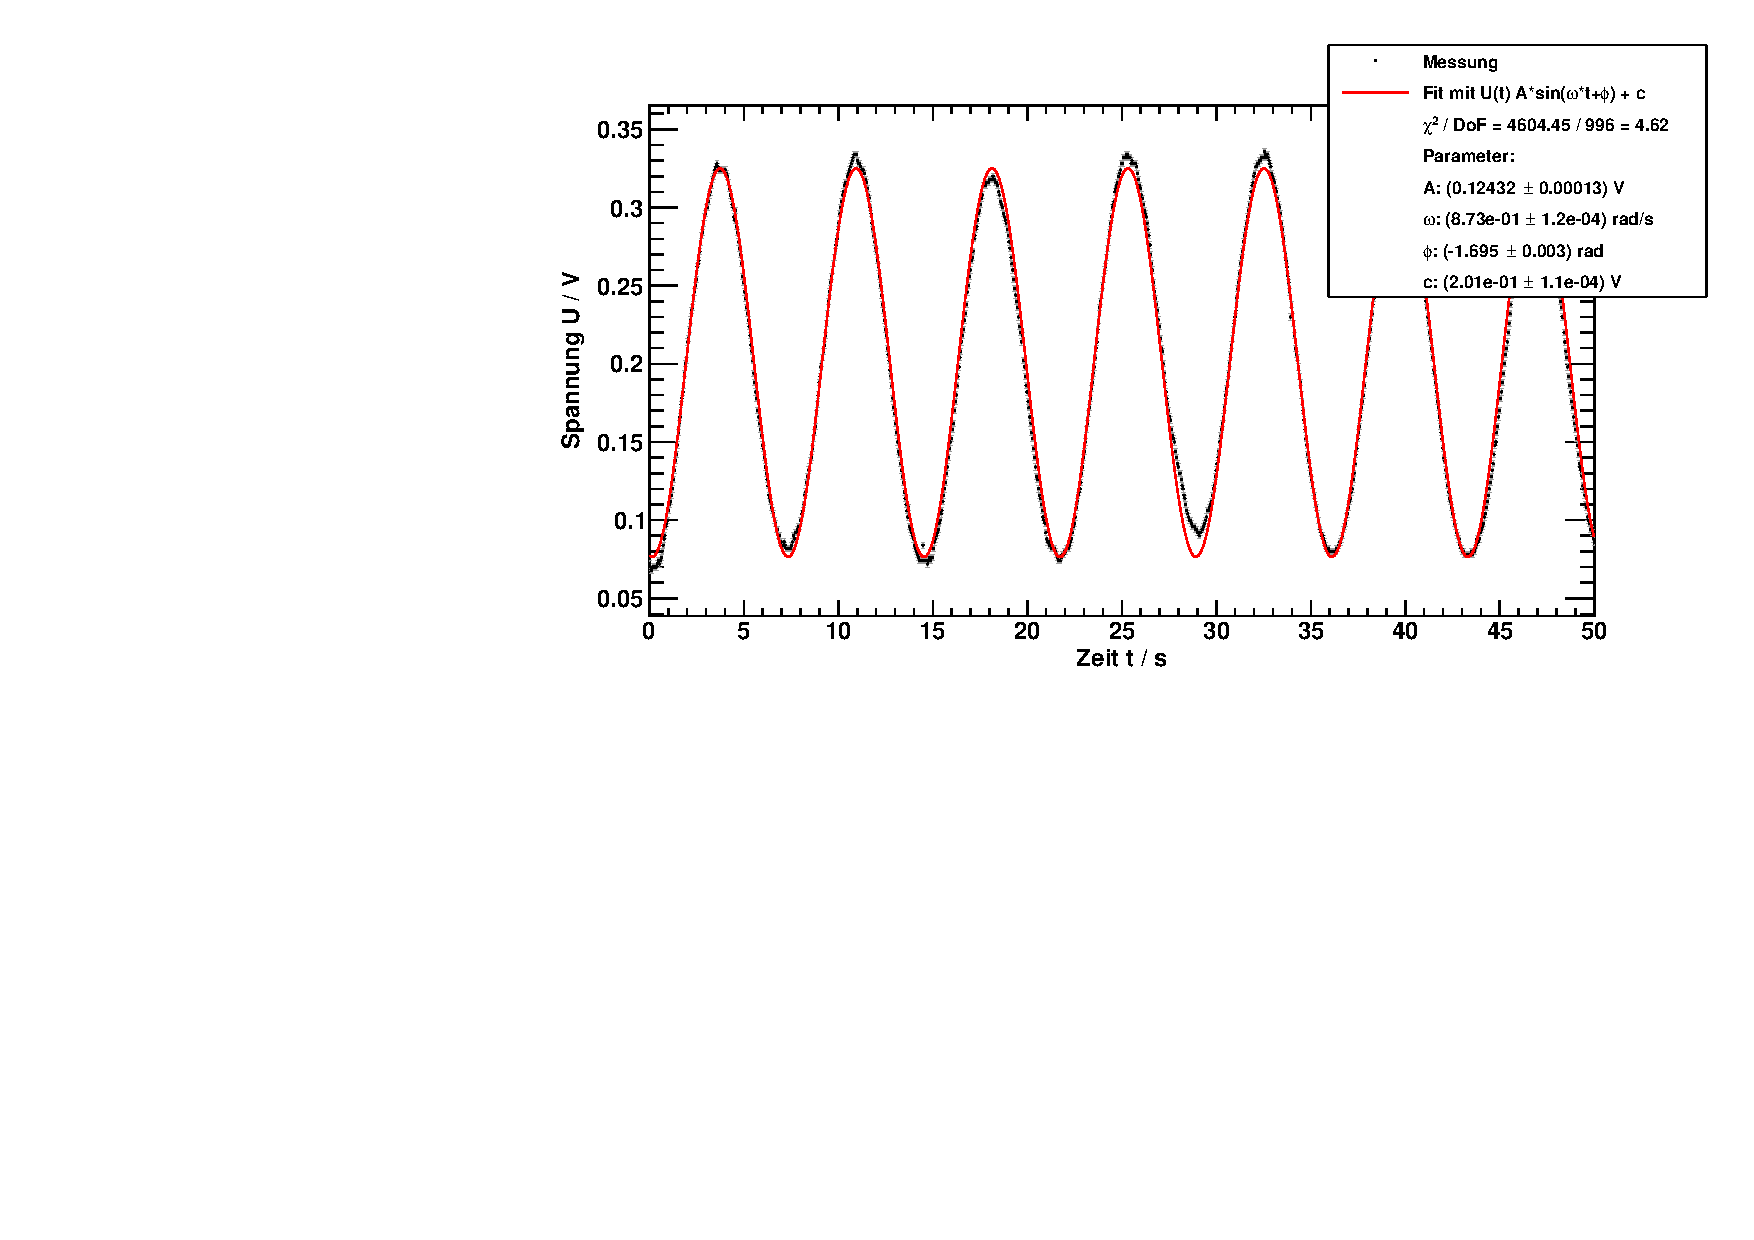
\includegraphics[width=0.64\textwidth]{../img/fit_Spule_R2.pdf}
  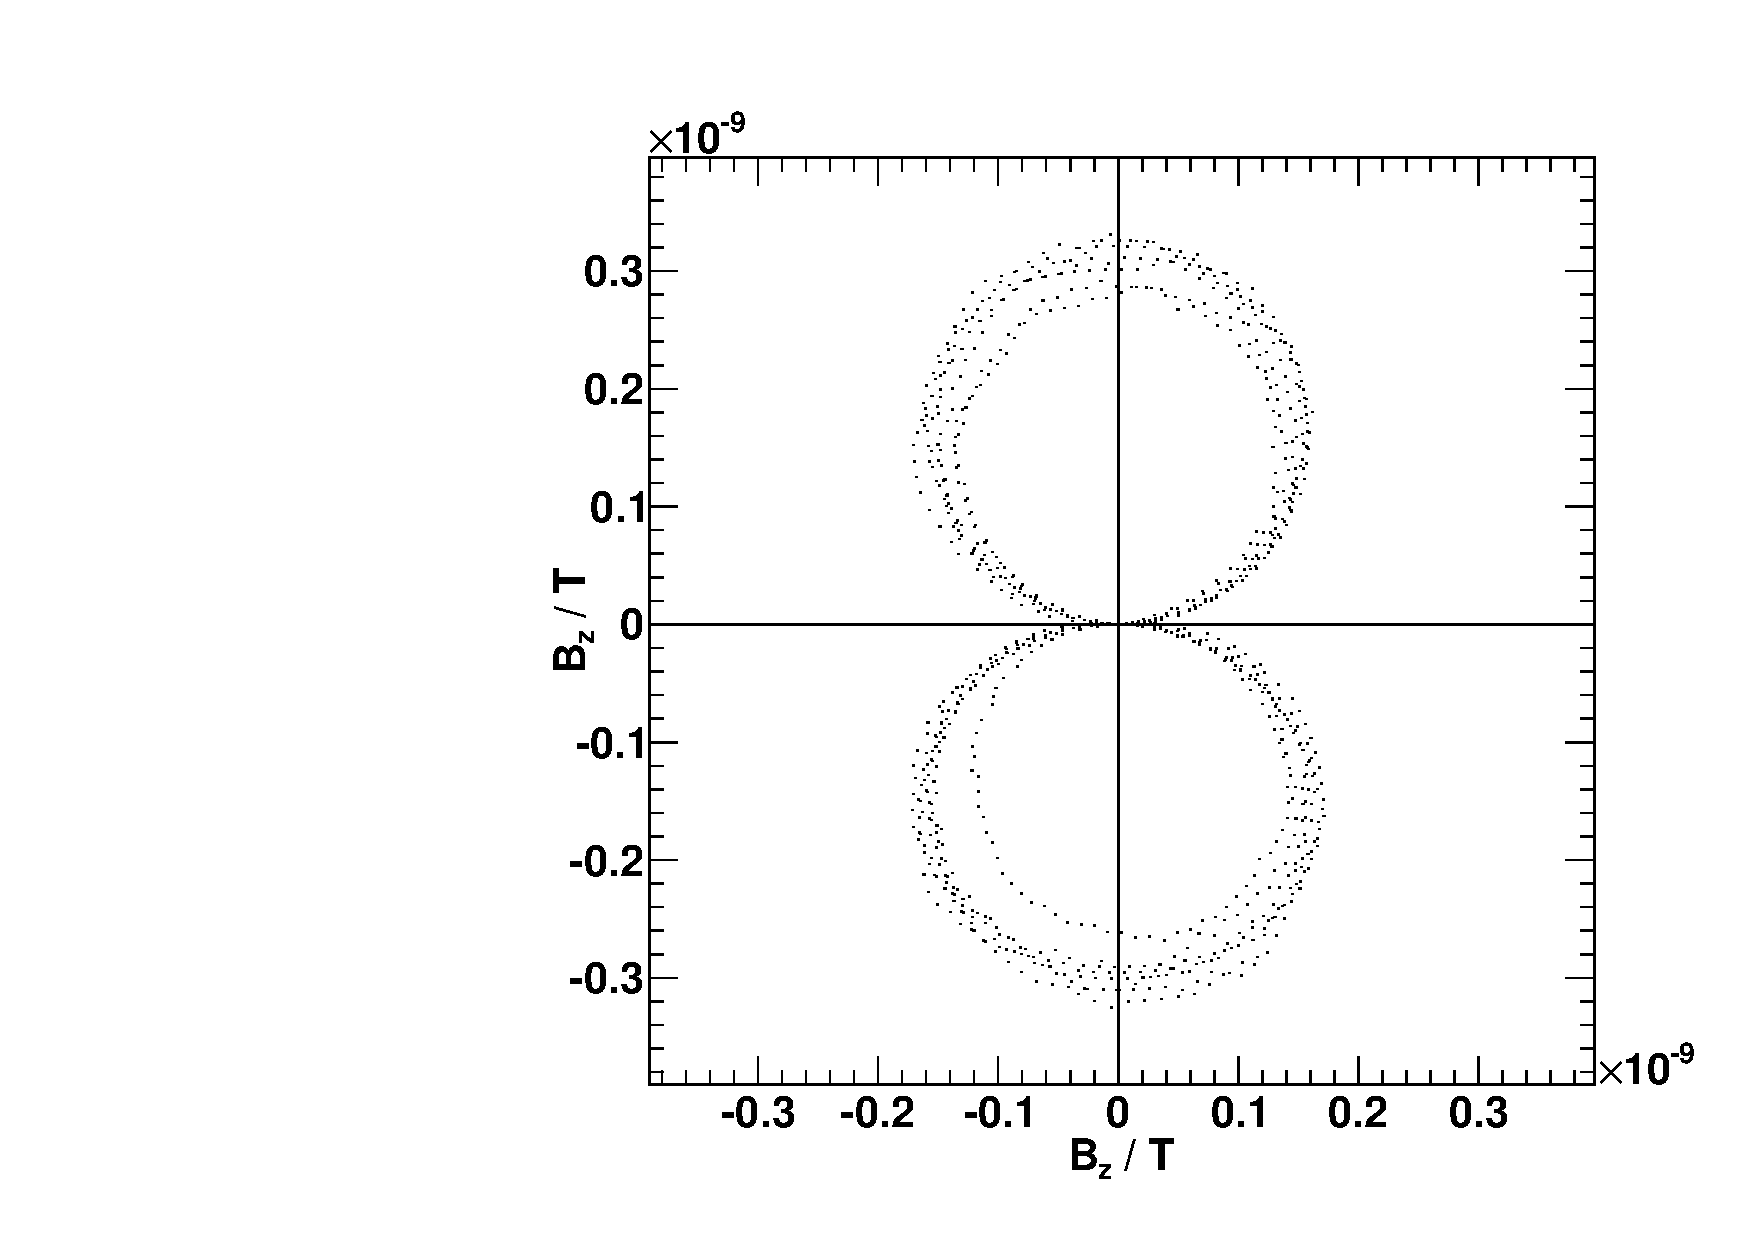
\includegraphics[width=0.35\textwidth]{../img/polar_Spule_R2.pdf}
  \caption{caption}
  \label{img:R2}
\end{center}
\end{figure}

\begin{figure}[H]
\begin{center}
  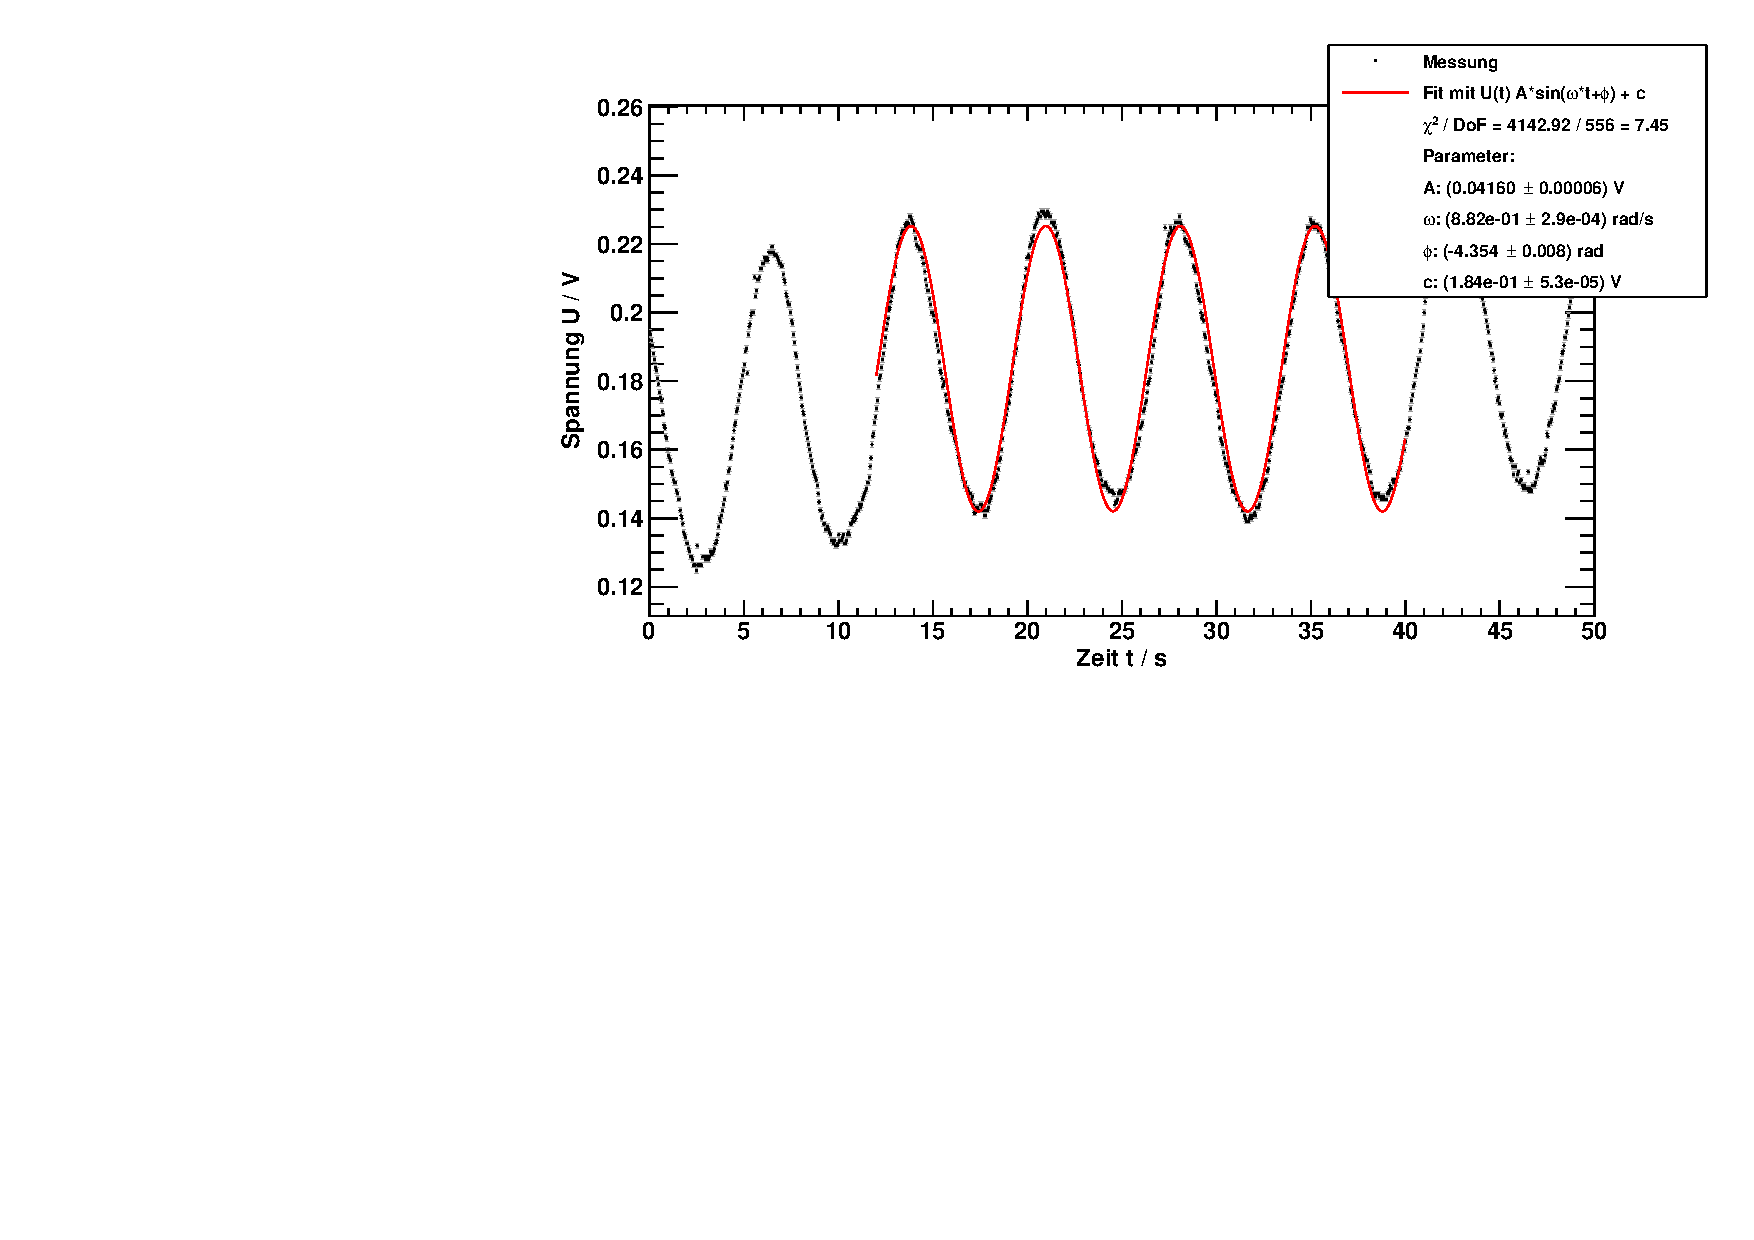
\includegraphics[width=0.64\textwidth]{../img/fit_Spule_R3.pdf}
  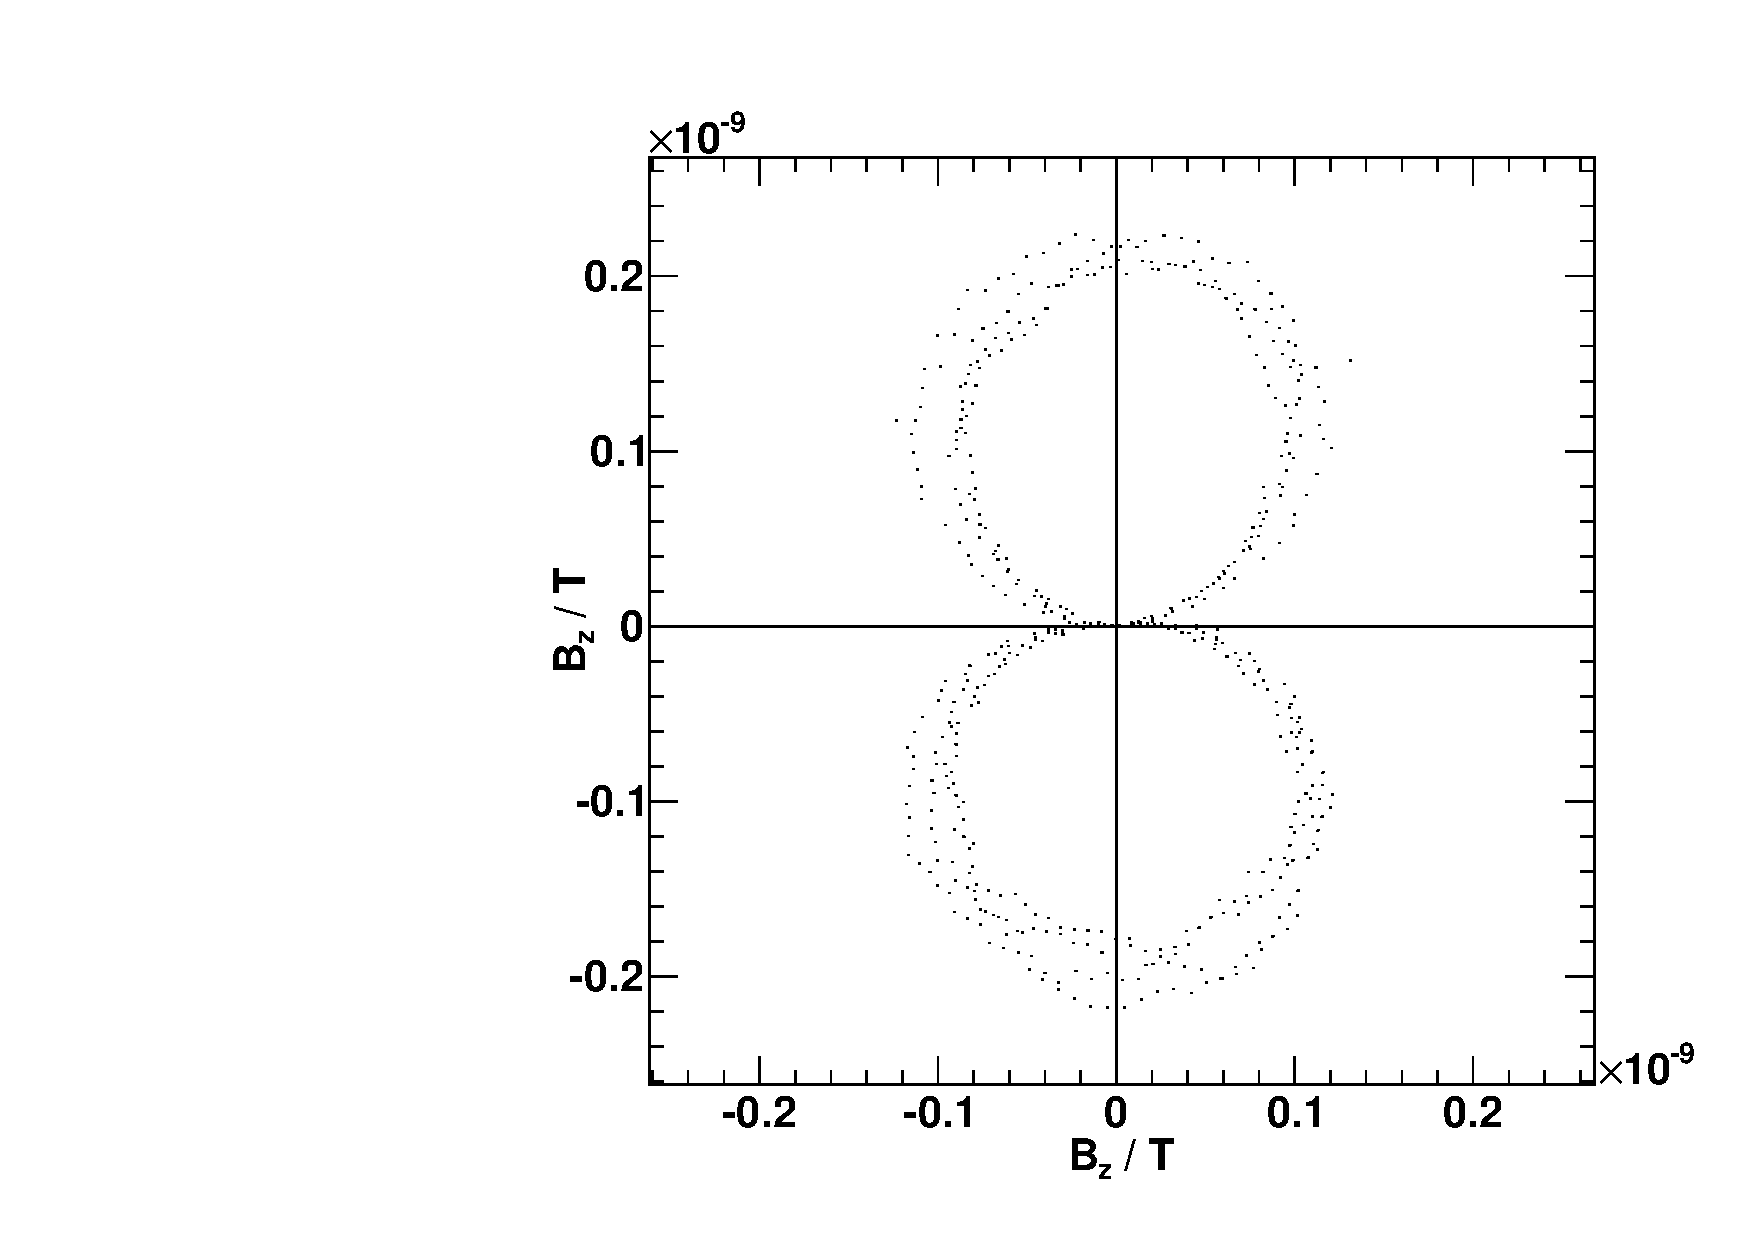
\includegraphics[width=0.35\textwidth]{../img/polar_Spule_R3.pdf}
  \caption{caption}
  \label{img:R3}
\end{center}
\end{figure}

\begin{figure}[H]
\begin{center}
  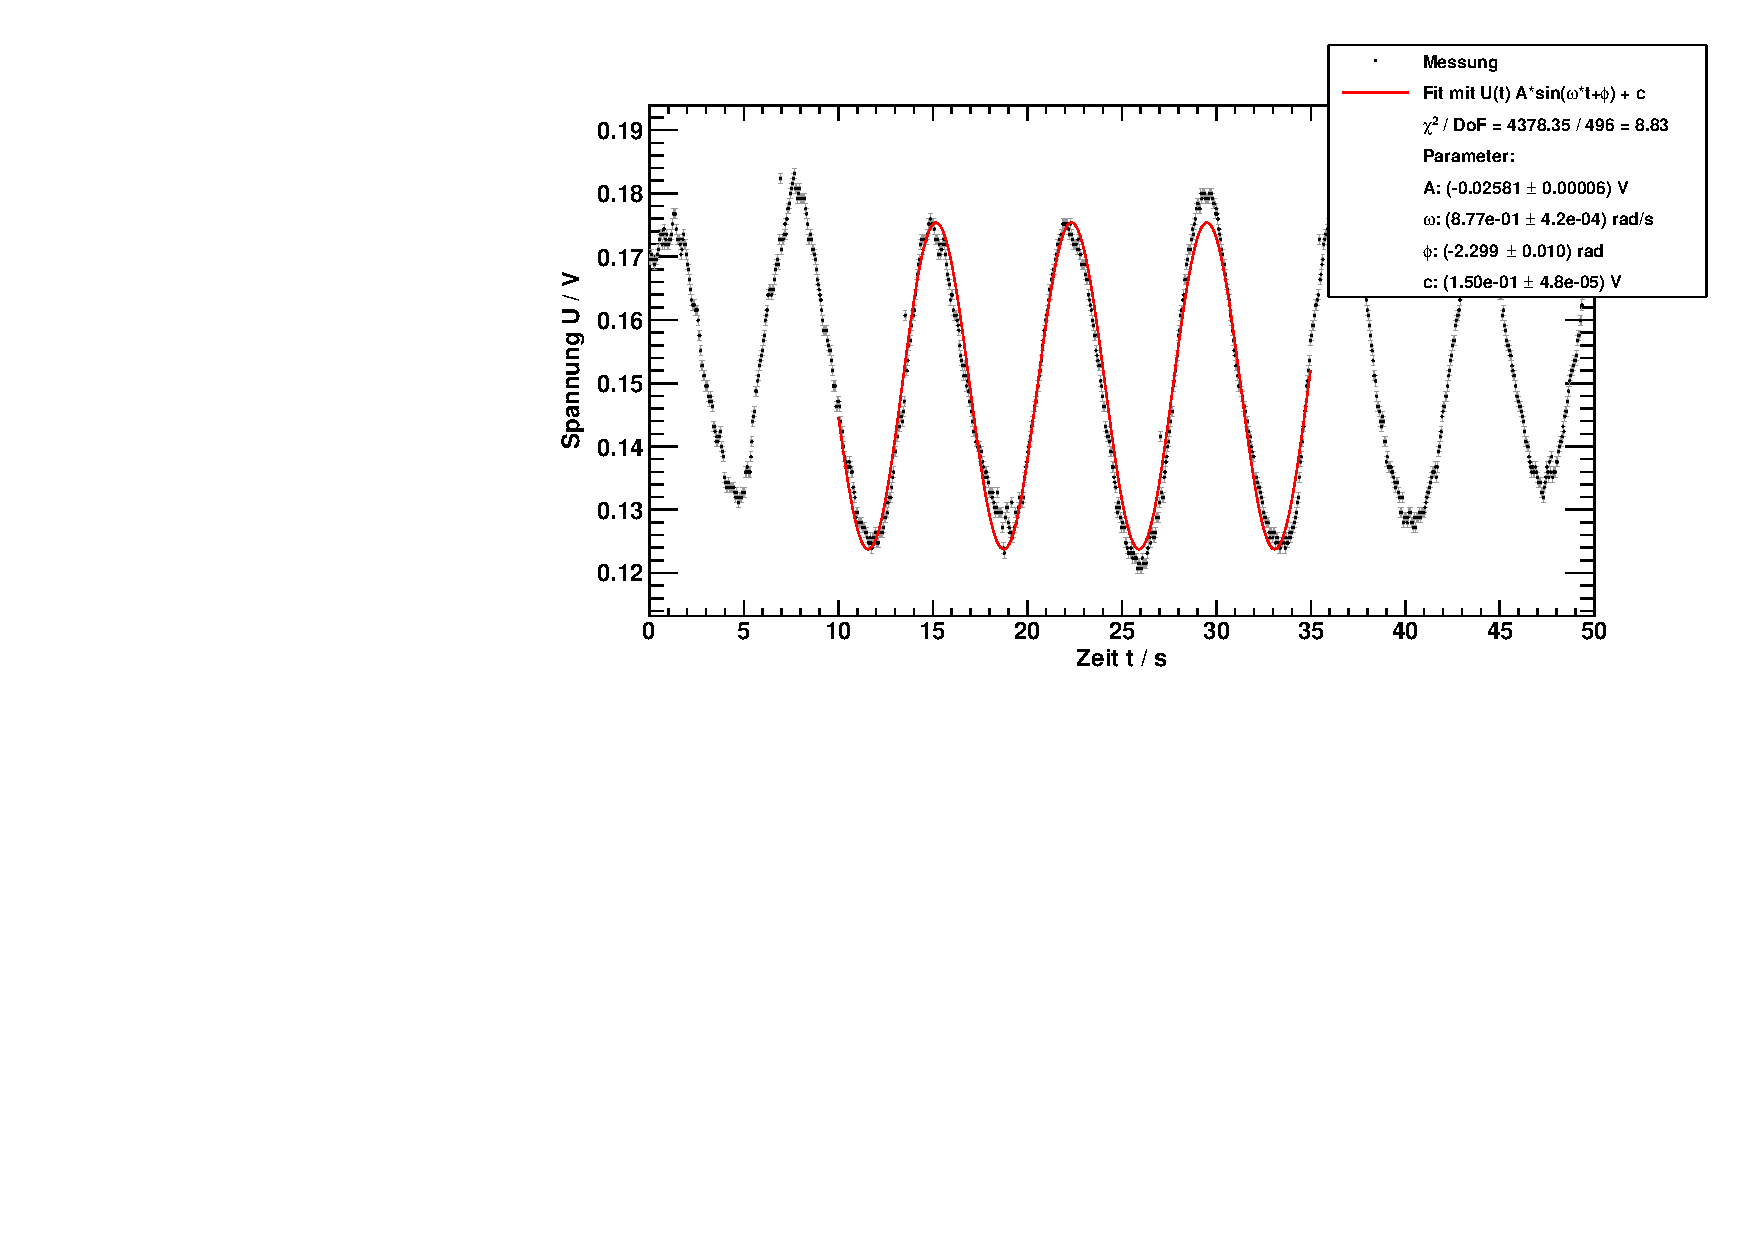
\includegraphics[width=0.64\textwidth]{../img/fit_Spule_R4.pdf}
  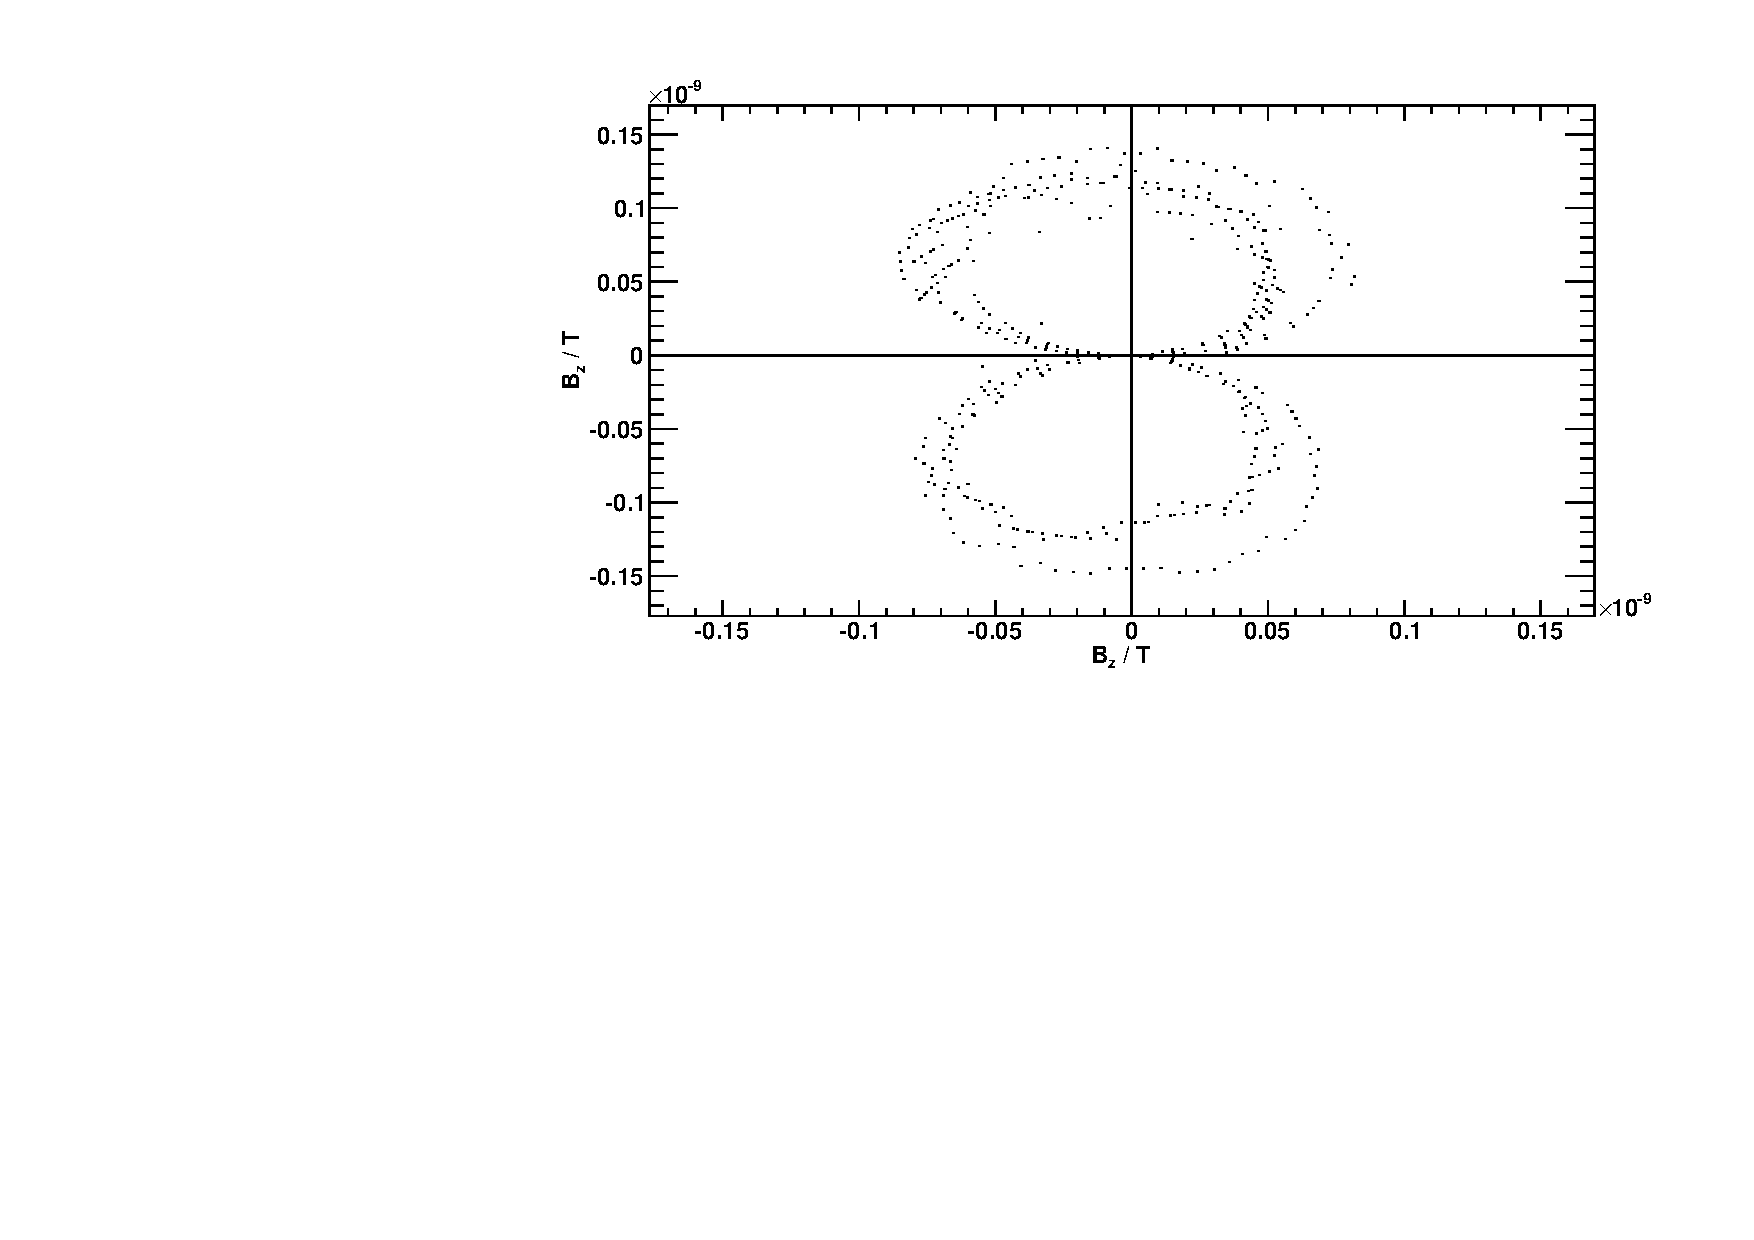
\includegraphics[width=0.35\textwidth]{../img/polar_Spule_R4.pdf}
  \caption{caption}
  \label{img:R4}
\end{center}
\end{figure}

\begin{figure}[H]
\begin{center}
  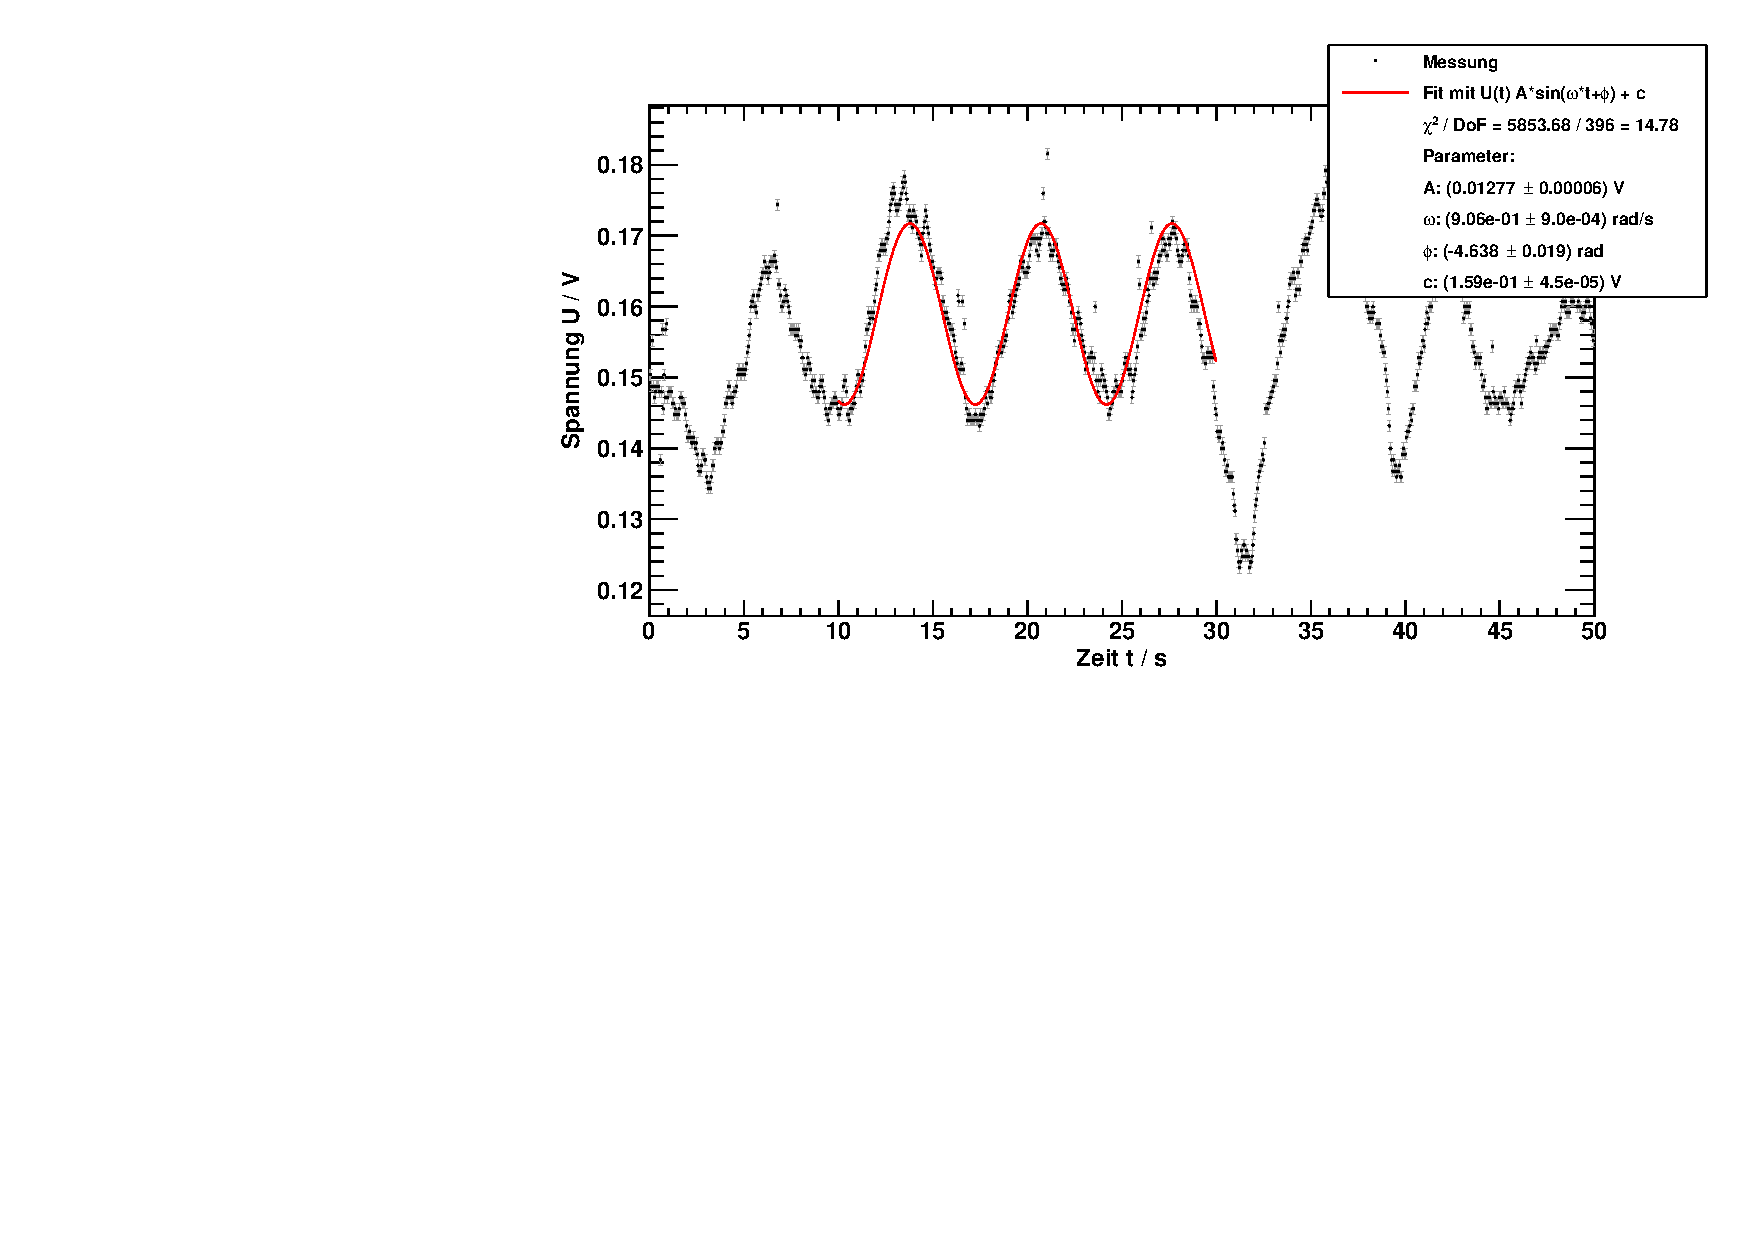
\includegraphics[width=0.64\textwidth]{../img/fit_Spule_R5_1.pdf}
  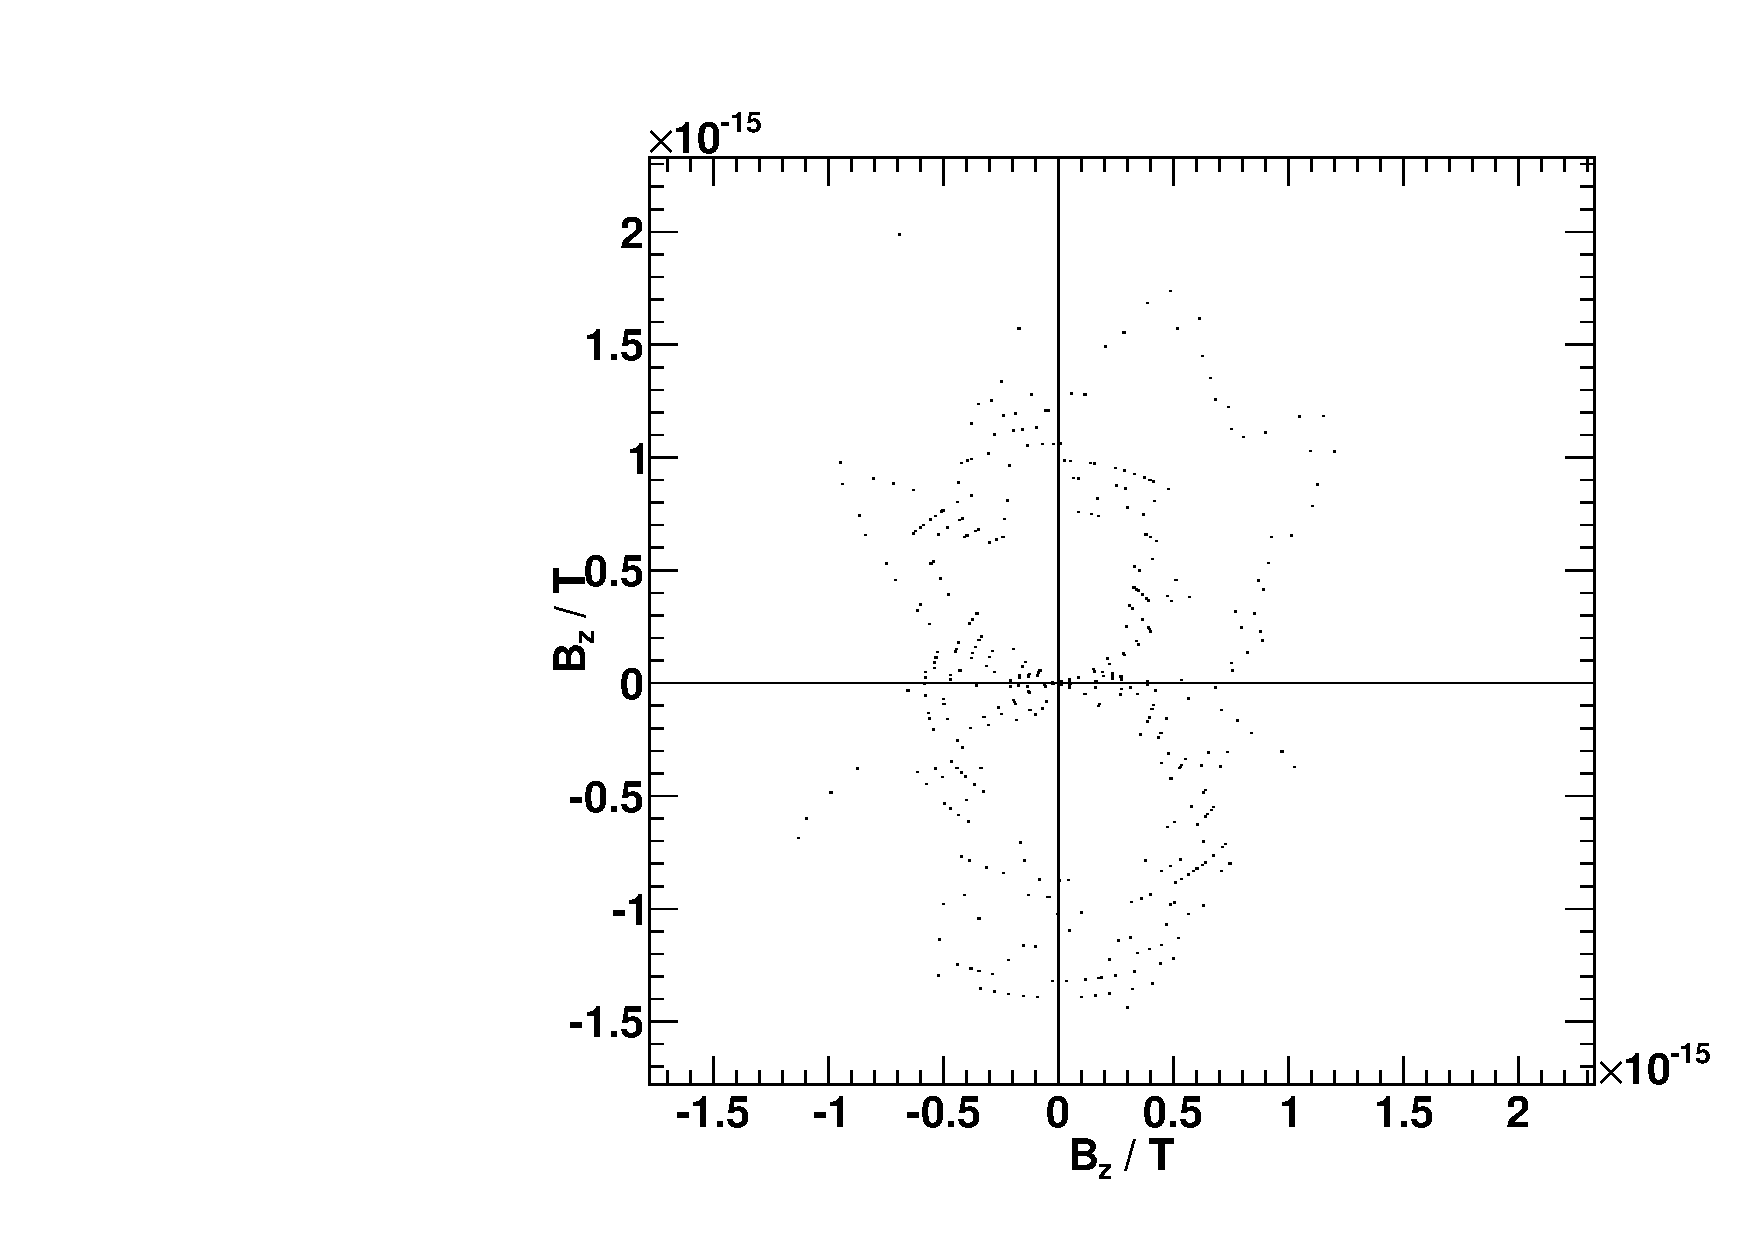
\includegraphics[width=0.35\textwidth]{../img/polar_Spule_R5_1.pdf}
  \caption{caption}
  \label{img:R5}
\end{center}
\end{figure}

\subsubsection{Berechnung aus der Geometrie der Leiterschleife}

\subsubsection{Vergleich}





\subsection{Vermessung des Magnetfelder verschiedener Proben}

\subsubsection{Untergrund}
\autoref{img:underground} zeigt das \emph{SQUID}-Signal bei ausgeschaltetem Motor, ohne Probe.
Es ist keine Periodizität des Signals zu erkennen. Die Schwankungen sind statistisch
und werden vermutlich durch wechselnde Magnetfelder von elektrischen Verbrauchern in der Umgebung verursacht.
Ein derartiges Untergrundrauschen mit 10\,mV bis 20\,mV Amplitude
ist allen Messungen überlagert und führt bei geringen Signalamplituden zu
Deformation und Drift der Messsignale.

\begin{figure}[H]
\begin{center}
  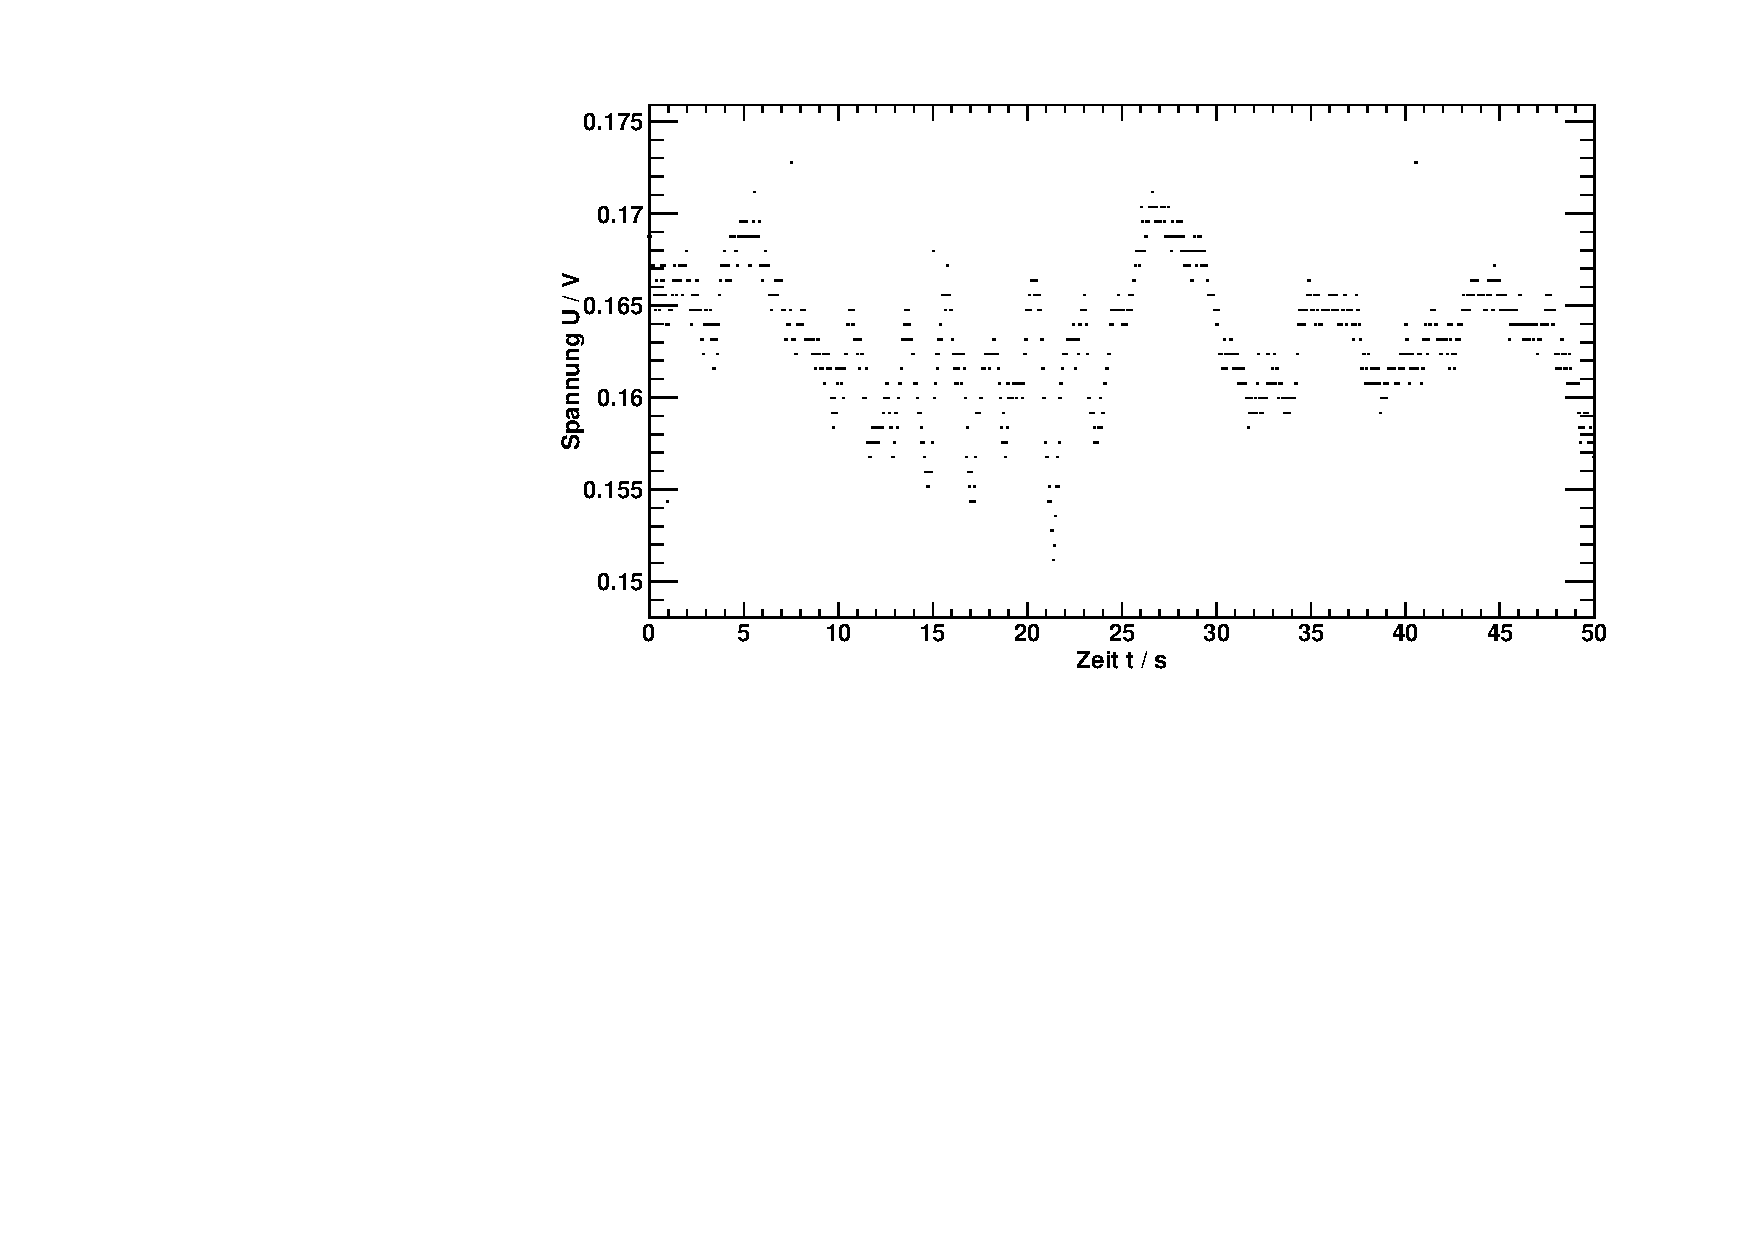
\includegraphics[width=0.8\textwidth]{../img/Untergrund.pdf}
  \caption{\emph{SQUID}-Signal ohne Probe, bei ausgeschaltetem Motor.}
  \label{img:underground}
\end{center}
\end{figure}



\subsubsection{Probenhalter}
Eine weitere Untergrundmessung ohne Probe wurde mit rotierendem Probenhalter durchgeführt.
Hier wird ein periodisches Signal mit ca. 40\,mV Amplitude gemessen.
Der Probenhalter ist also leicht magnetisch.\\
Zur Erstellung des Polarplots wurde der Mittelwert über die Winkelgeschwindigkeiten gebildet,
die aus den Sinusfits gewonnen wurden.
Im Polarplot ist keine deutliche Winkelabhängigkeit zu erkennen.



\begin{figure}[H]
\begin{center}
  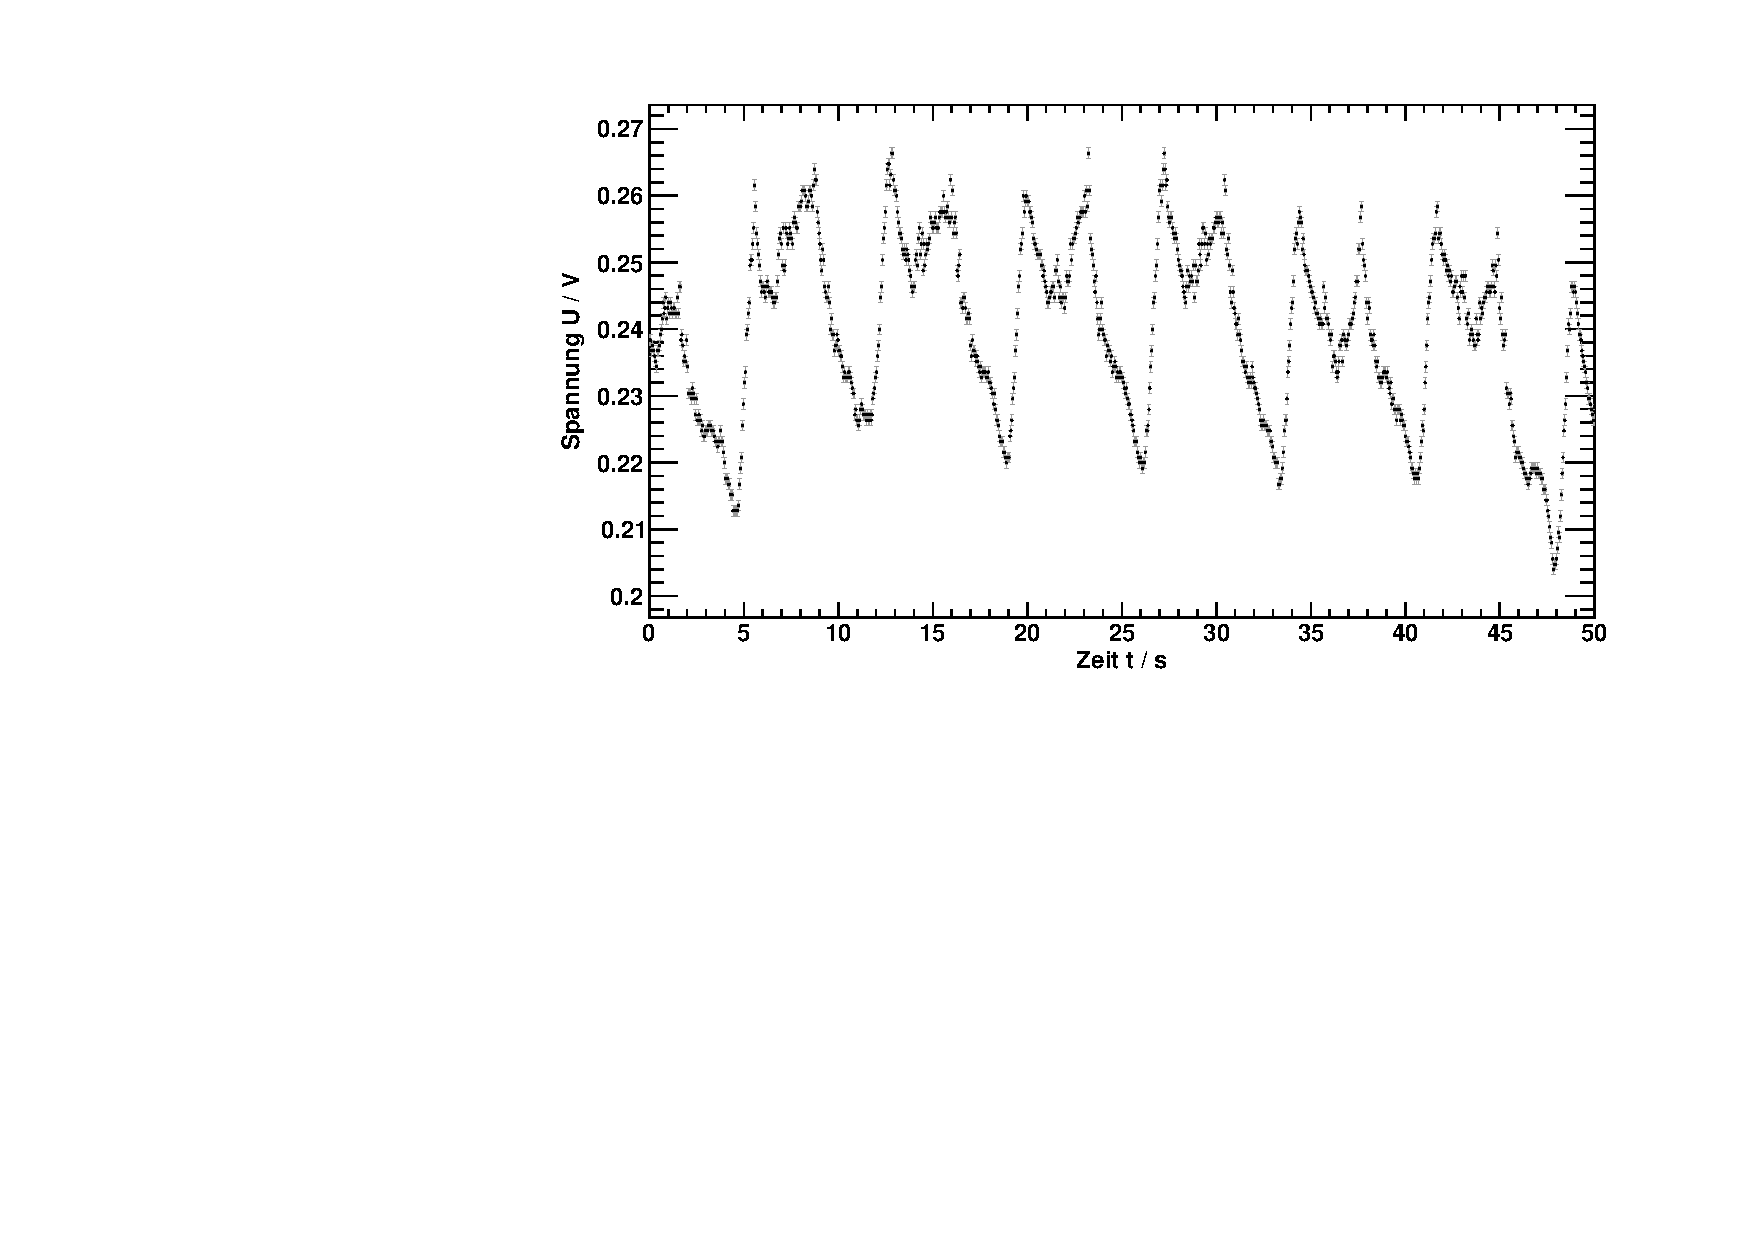
\includegraphics[width=0.64\textwidth]{../img/emptyHolder.pdf}
  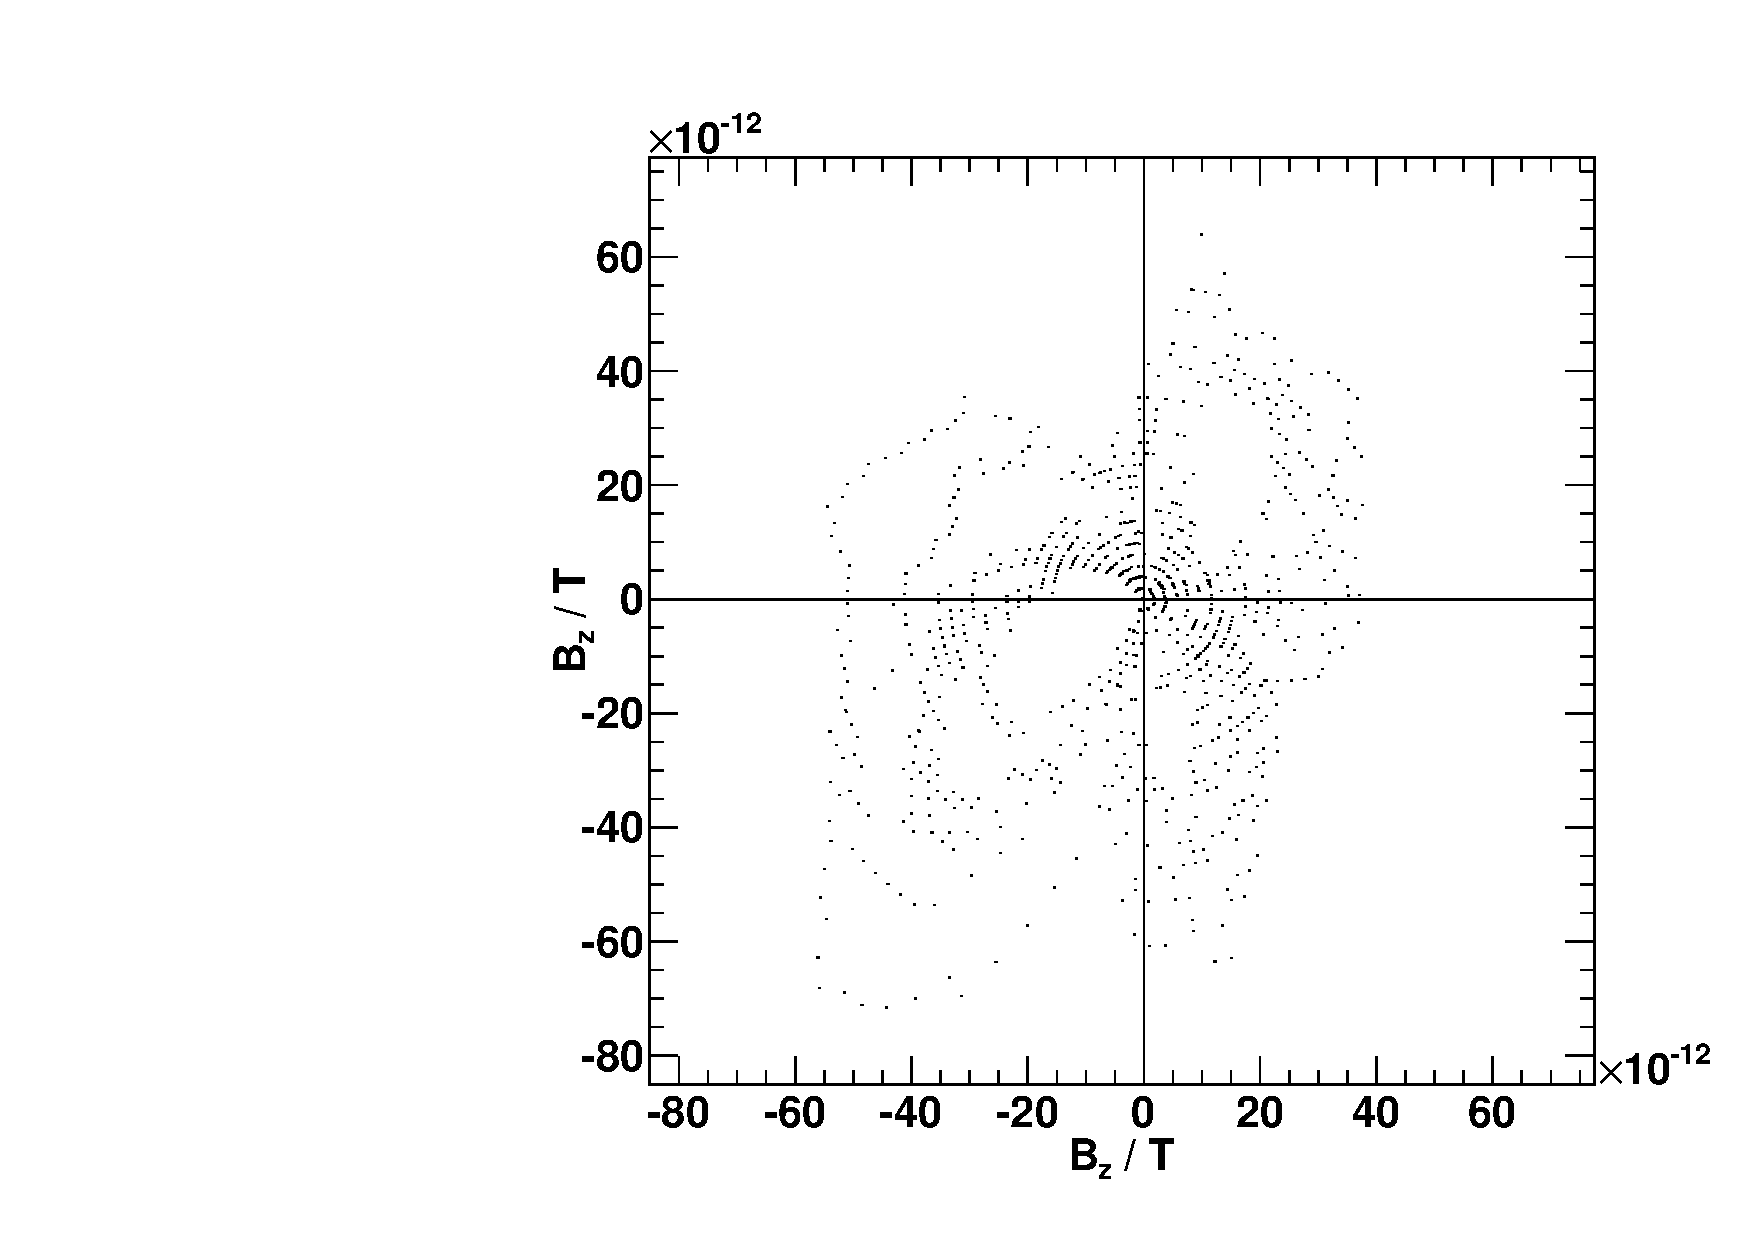
\includegraphics[width=0.35\textwidth]{../img/polar_emptyHolder.pdf}
  \caption{\emph{SQUID}-Signal bei leerem, rotierendem Probenhalter. Es ist eine leichte Magnetisierung des
  Probenhalters erkennbar.}
  \label{img:holder}
\end{center}
\end{figure}





\subsubsection{Stabmagnet}
\begin{figure}[H]
\begin{center}
  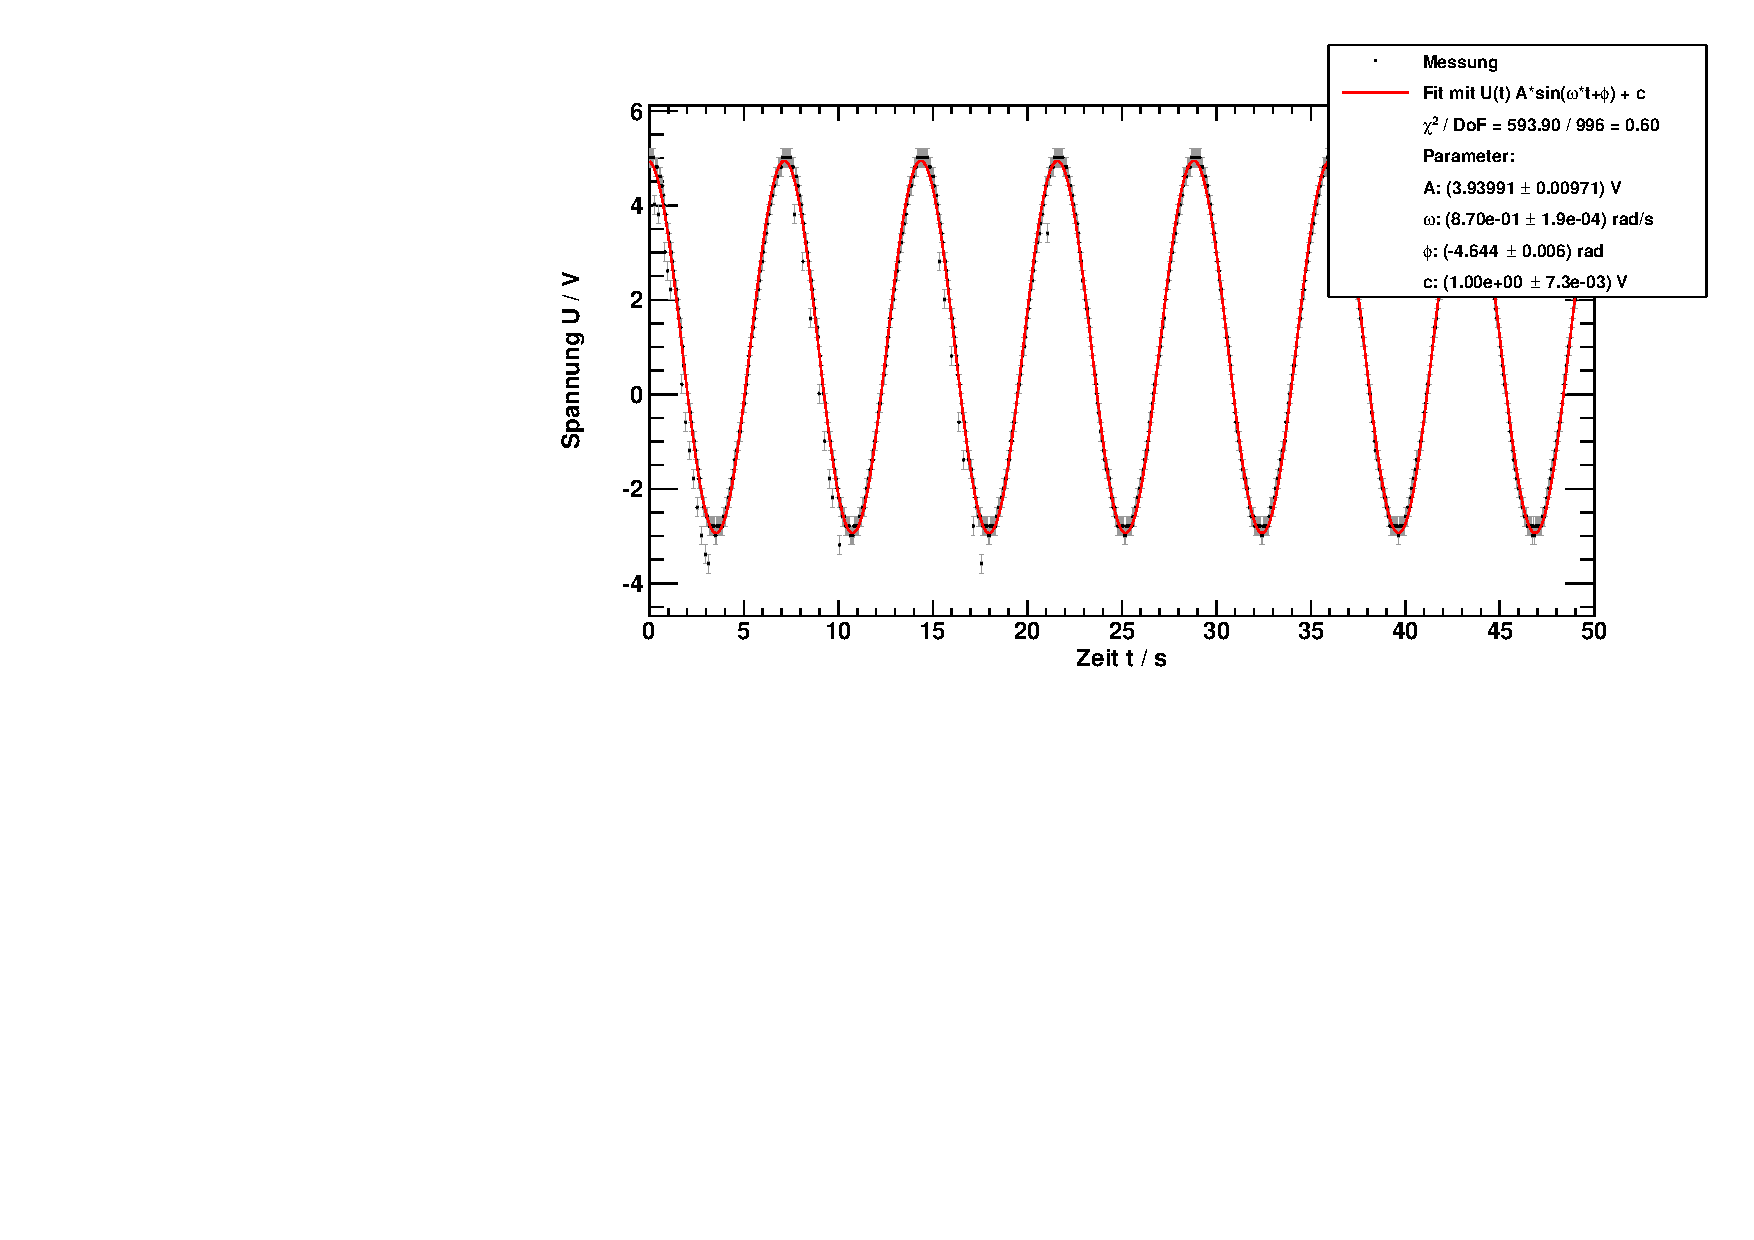
\includegraphics[width=0.64\textwidth]{../img/fit_Magnet.pdf}
  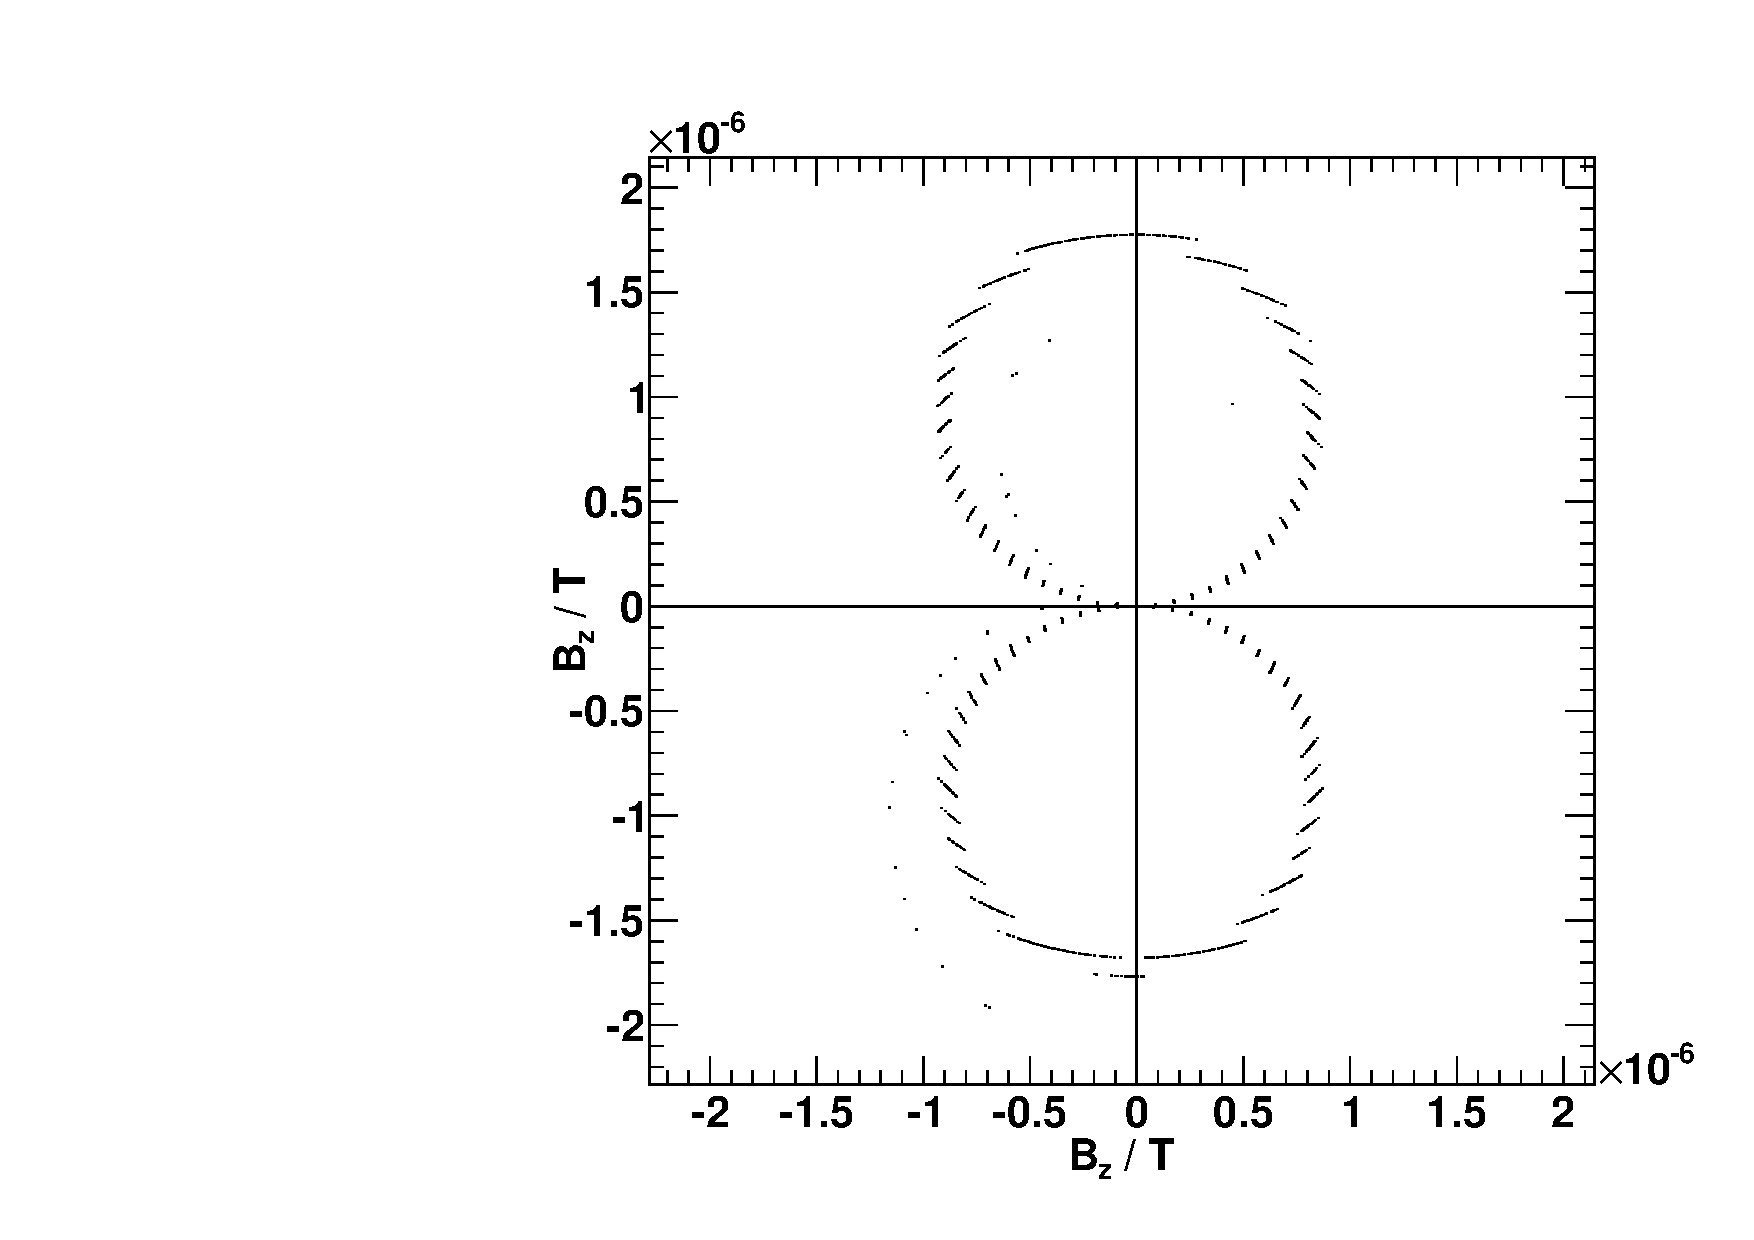
\includegraphics[width=0.35\textwidth]{../img/polar_Magnet.pdf}
  \caption{Bestimmung des Magnetfelds eines kleinen Stabmagneten und Fit mit Sinusfunktion.}
  \label{img:magnet}
\end{center}
\end{figure}
Die Messung am Stabmagneten wurde gemäß \autoref{eq:fit} gefittet.
Für die Amplitude der Schwingung erhält man
\begin{equation}
\label{}
A_{\text{St}}=(3.9399 \pm 0.0010)\, \text{V} \ \, .
\end{equation}
Daraus folgt nach \autoref{eq:AtoB} für die maximale Magnetfeldstärke des Stabmagneten
\begin{equation}
\label{}
B_{\text{St}} = (1.745 \pm 0.004)\,\text{\textmu T} \ \, .
\end{equation}
Auf dem Polarplot ist deutlich die Struktur des magnetischen Dipols zu erkennen.


\subsubsection{Magnet-Span}
\begin{figure}[H]
\begin{center}
  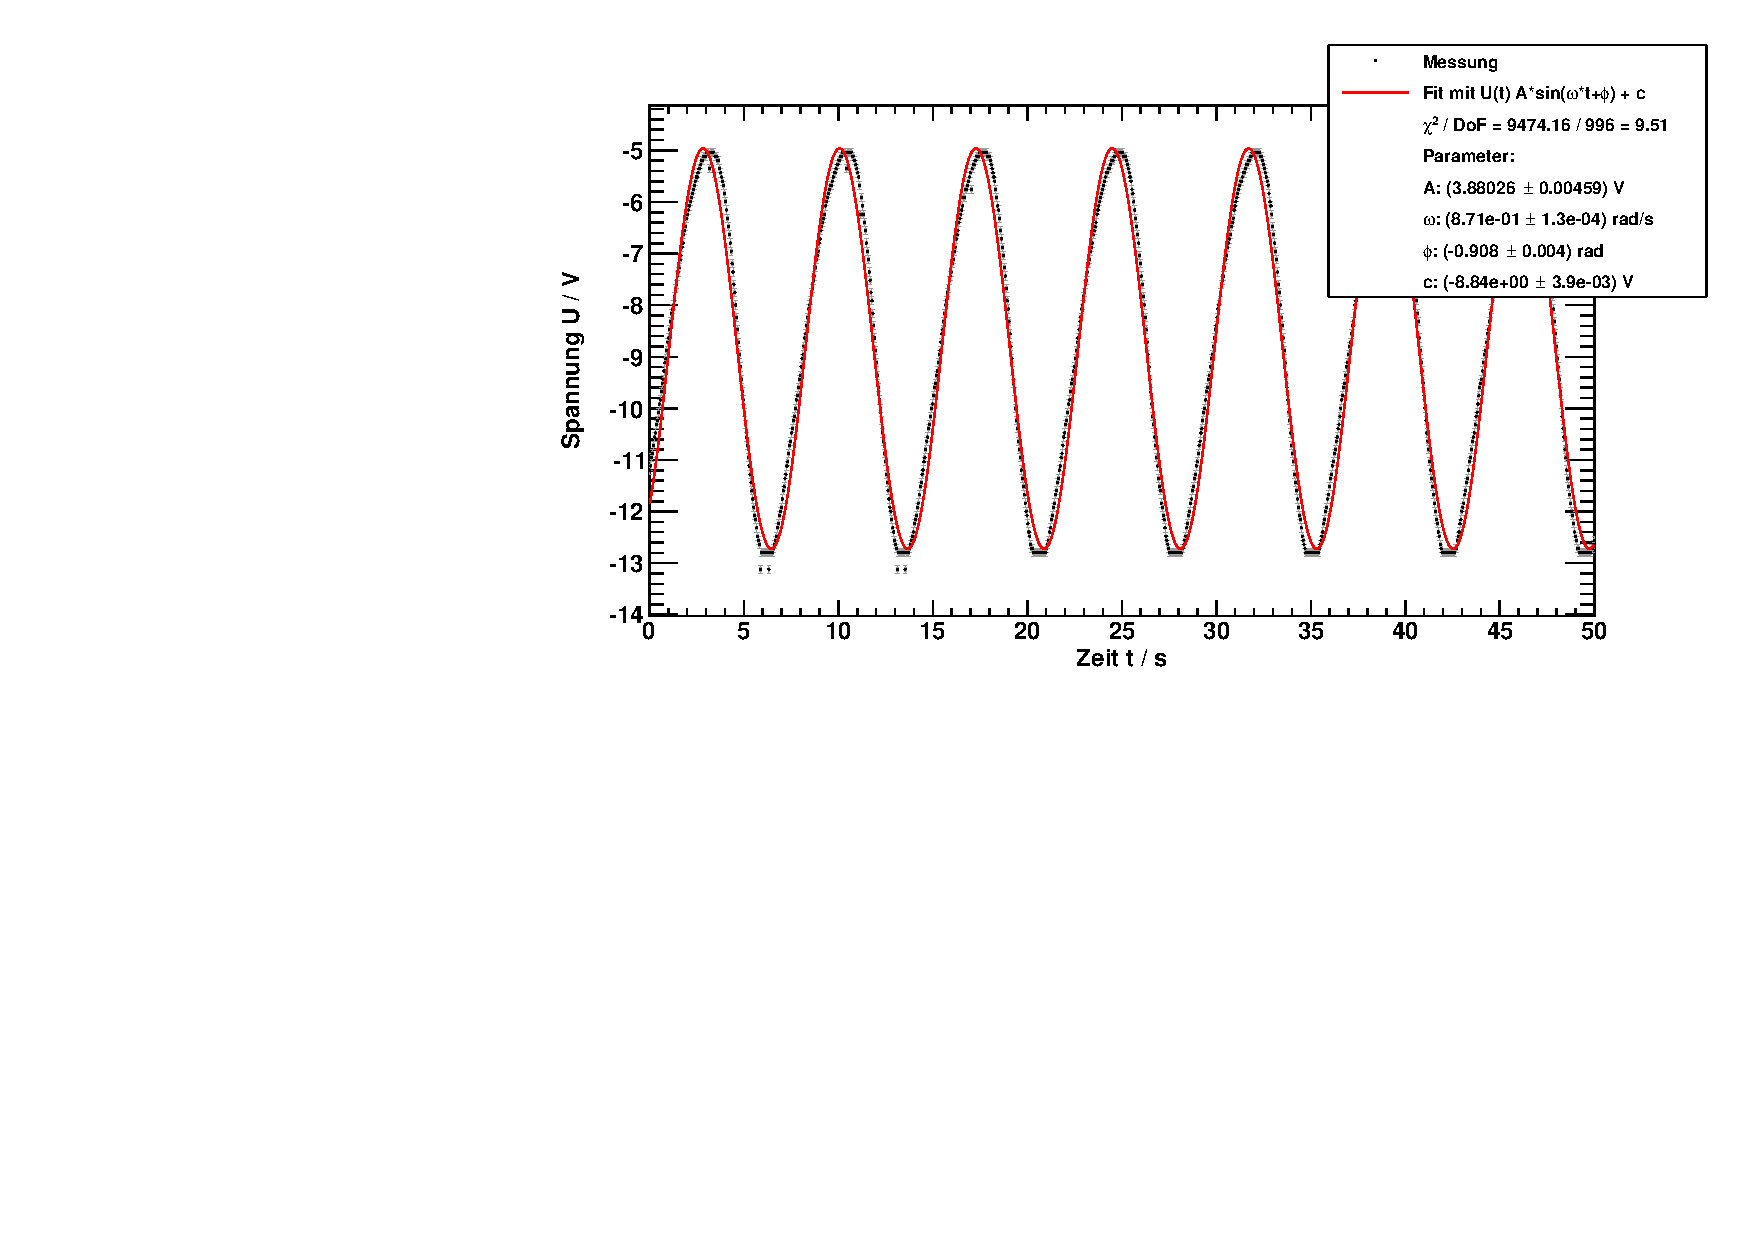
\includegraphics[width=0.64\textwidth]{../img/fit_Magnetspan_45grad.pdf}
  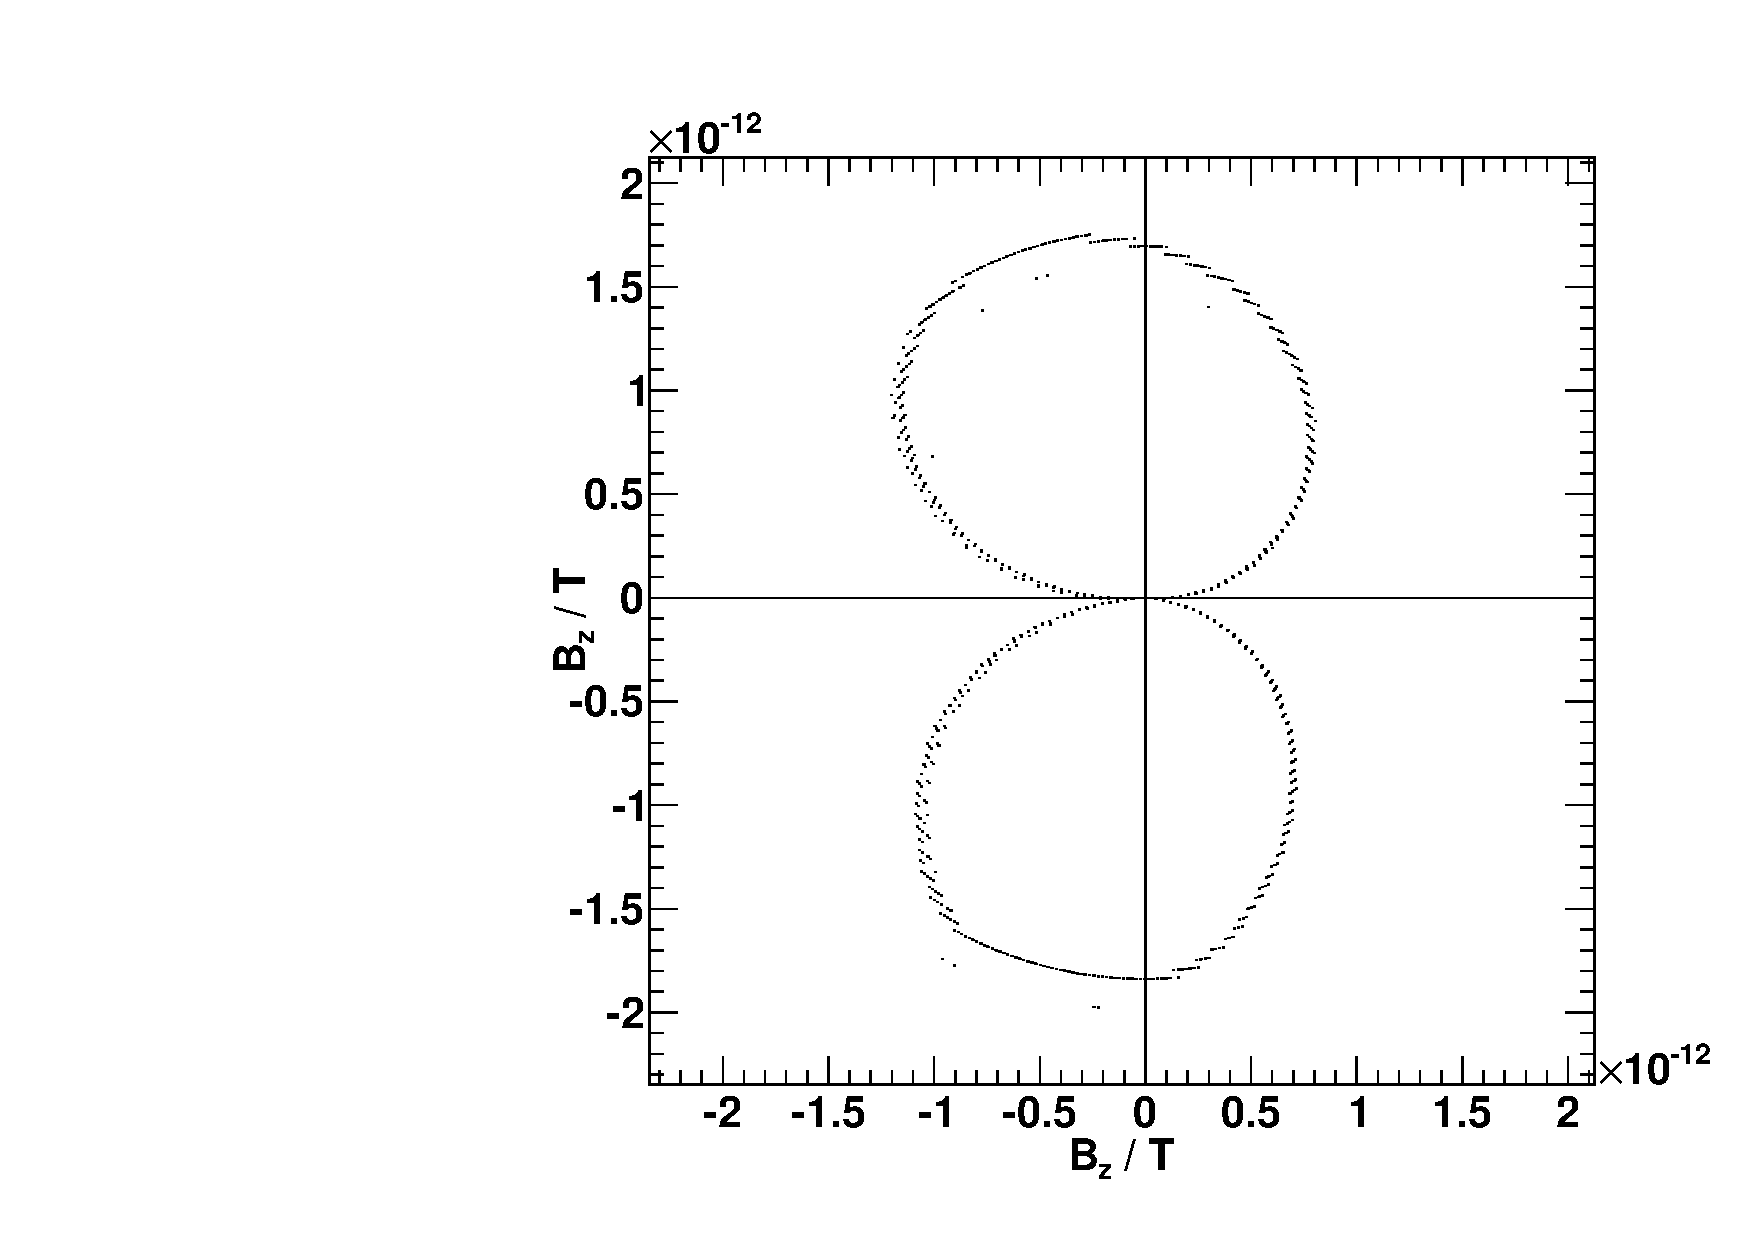
\includegraphics[width=0.35\textwidth]{../img/polar_Magnetspan_45grad.pdf}
  \caption{Bestimmung des Magnetfelds eines Magnetspans und Fit mit Sinusfunktion.}
  \label{img:magnetspan}
\end{center}
\end{figure}
Auch die Messung am Stabmagneten wurde gemäß \autoref{eq:fit} gefittet.
Für die Amplitude der Schwingung erhält man
\begin{equation}
\label{}
A_{\text{St}}=(3.880 \pm 0.005)\, \text{V} \ \, .
\end{equation}
Daraus folgt nach \autoref{eq:AtoB} für die maximale Magnetfeldstärke des Stabmagneten
\begin{equation}
\label{}
B_{\text{St}} = (94.96 \pm 0.11)\,\text{nT} \ \, .
\end{equation}
Obwohl die Spannungsamplitude hier fast genauso hoch ist wie bei der Messung am Stabmagneten,
ist das berechnete Magnetfeld viel kleiner. Dies liegt an den unterschiedlichen Widerständen,
die bei der Messung gewählt wurden.\\ 
Auf dem Polarplot ist ebenfalls deutlich die Struktur des magnetischen Dipols zu erkennen.


\subsubsection{Eisen-Span}
\begin{figure}[H]
\begin{center}
  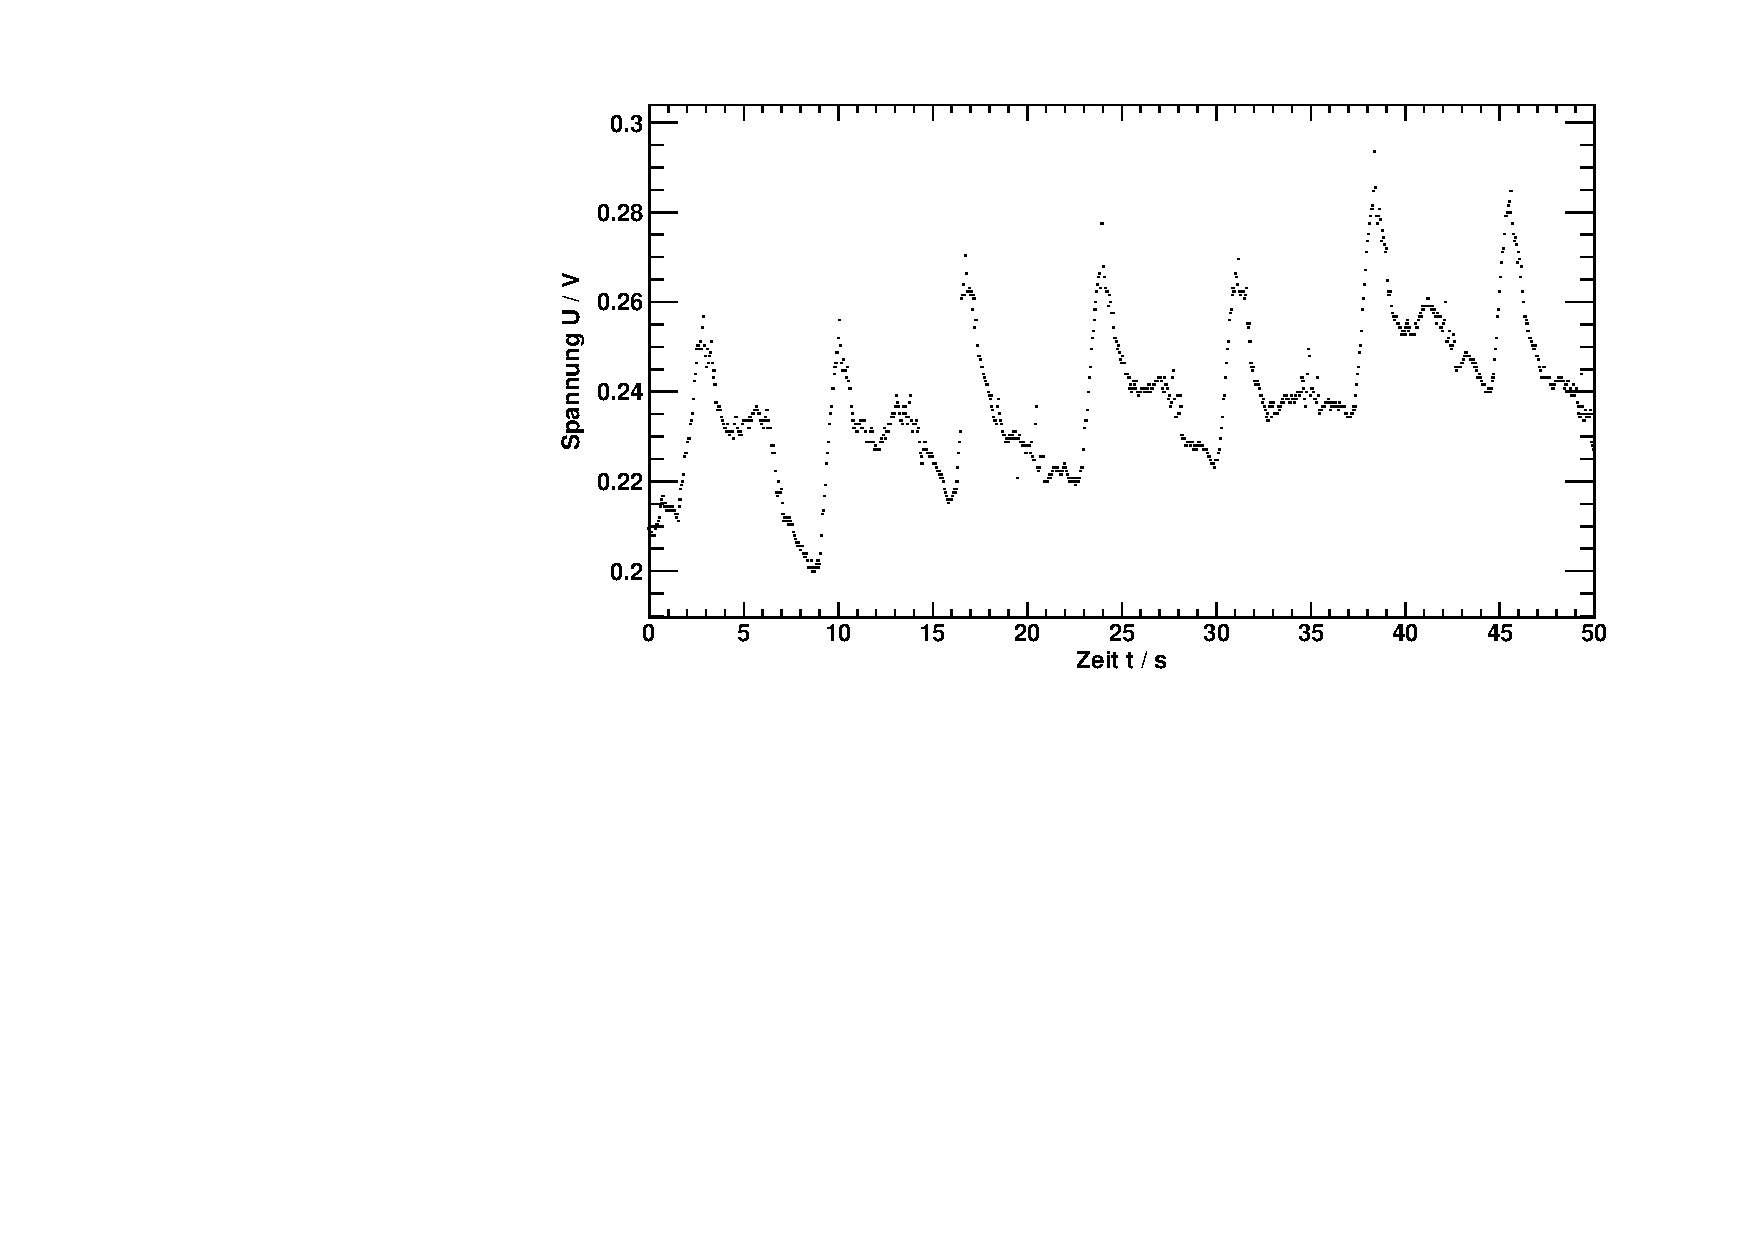
\includegraphics[width=0.64\textwidth]{../img/Fe-Span.pdf}
  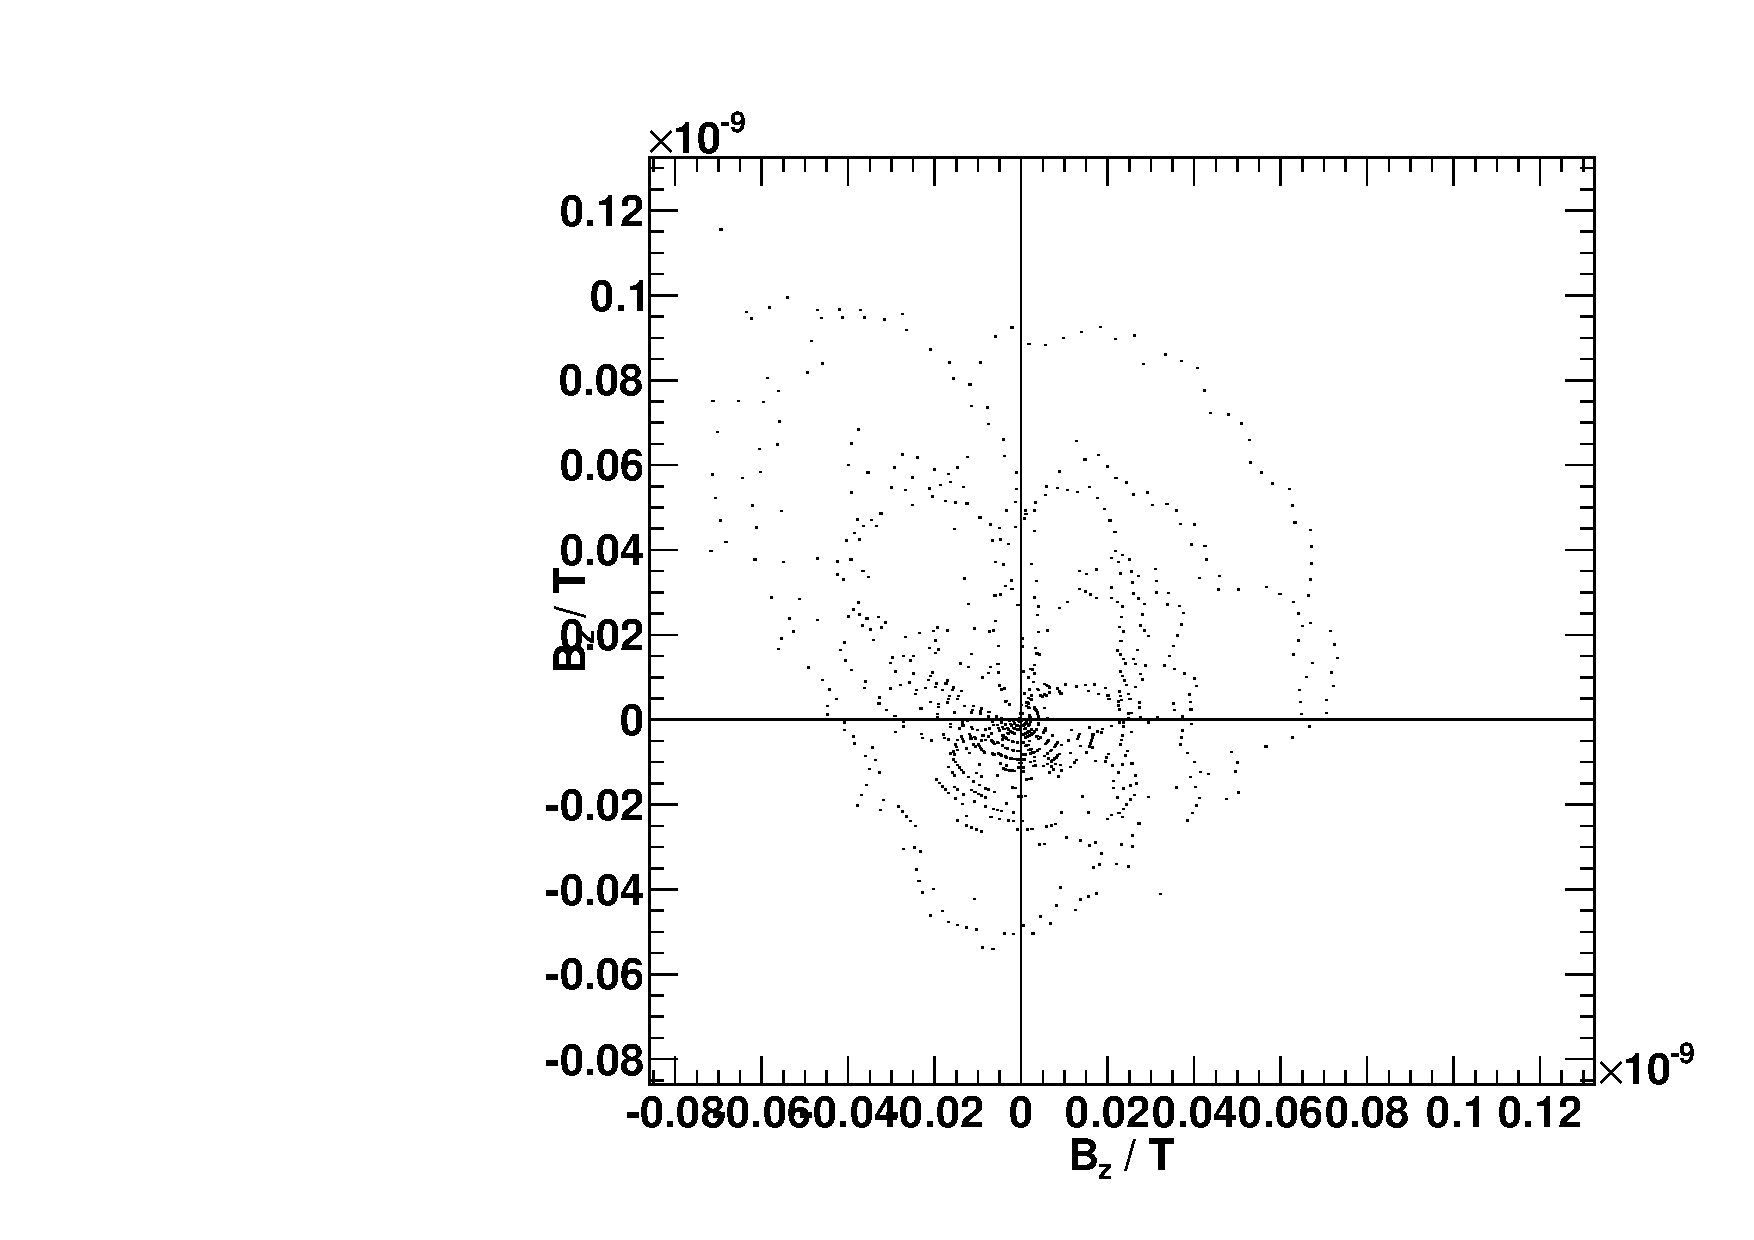
\includegraphics[width=0.35\textwidth]{../img/polar_Fe-Span.pdf}
  \caption{Bestimmung des Magnetfelds eines Eisenspans. Das periodische Signal stammt vermutlich
  vom magnetisierten Probenhalter (\autoref{img:holder}).}
  \label{img:fespan}
\end{center}
\end{figure}
Bei der Messung am Eisenspan ist keine Magnetisierung erkennbar.
Das periodische Signal mit 40\,mV Amplitude wird vermutlich durch den magnetisierten Probenhalter
verursacht (siehe oben).\\
Der Polarplot liefert hier keine eindeutige Aussage.


\subsubsection{Goldplättchen}
\begin{figure}[H]
\begin{center}
  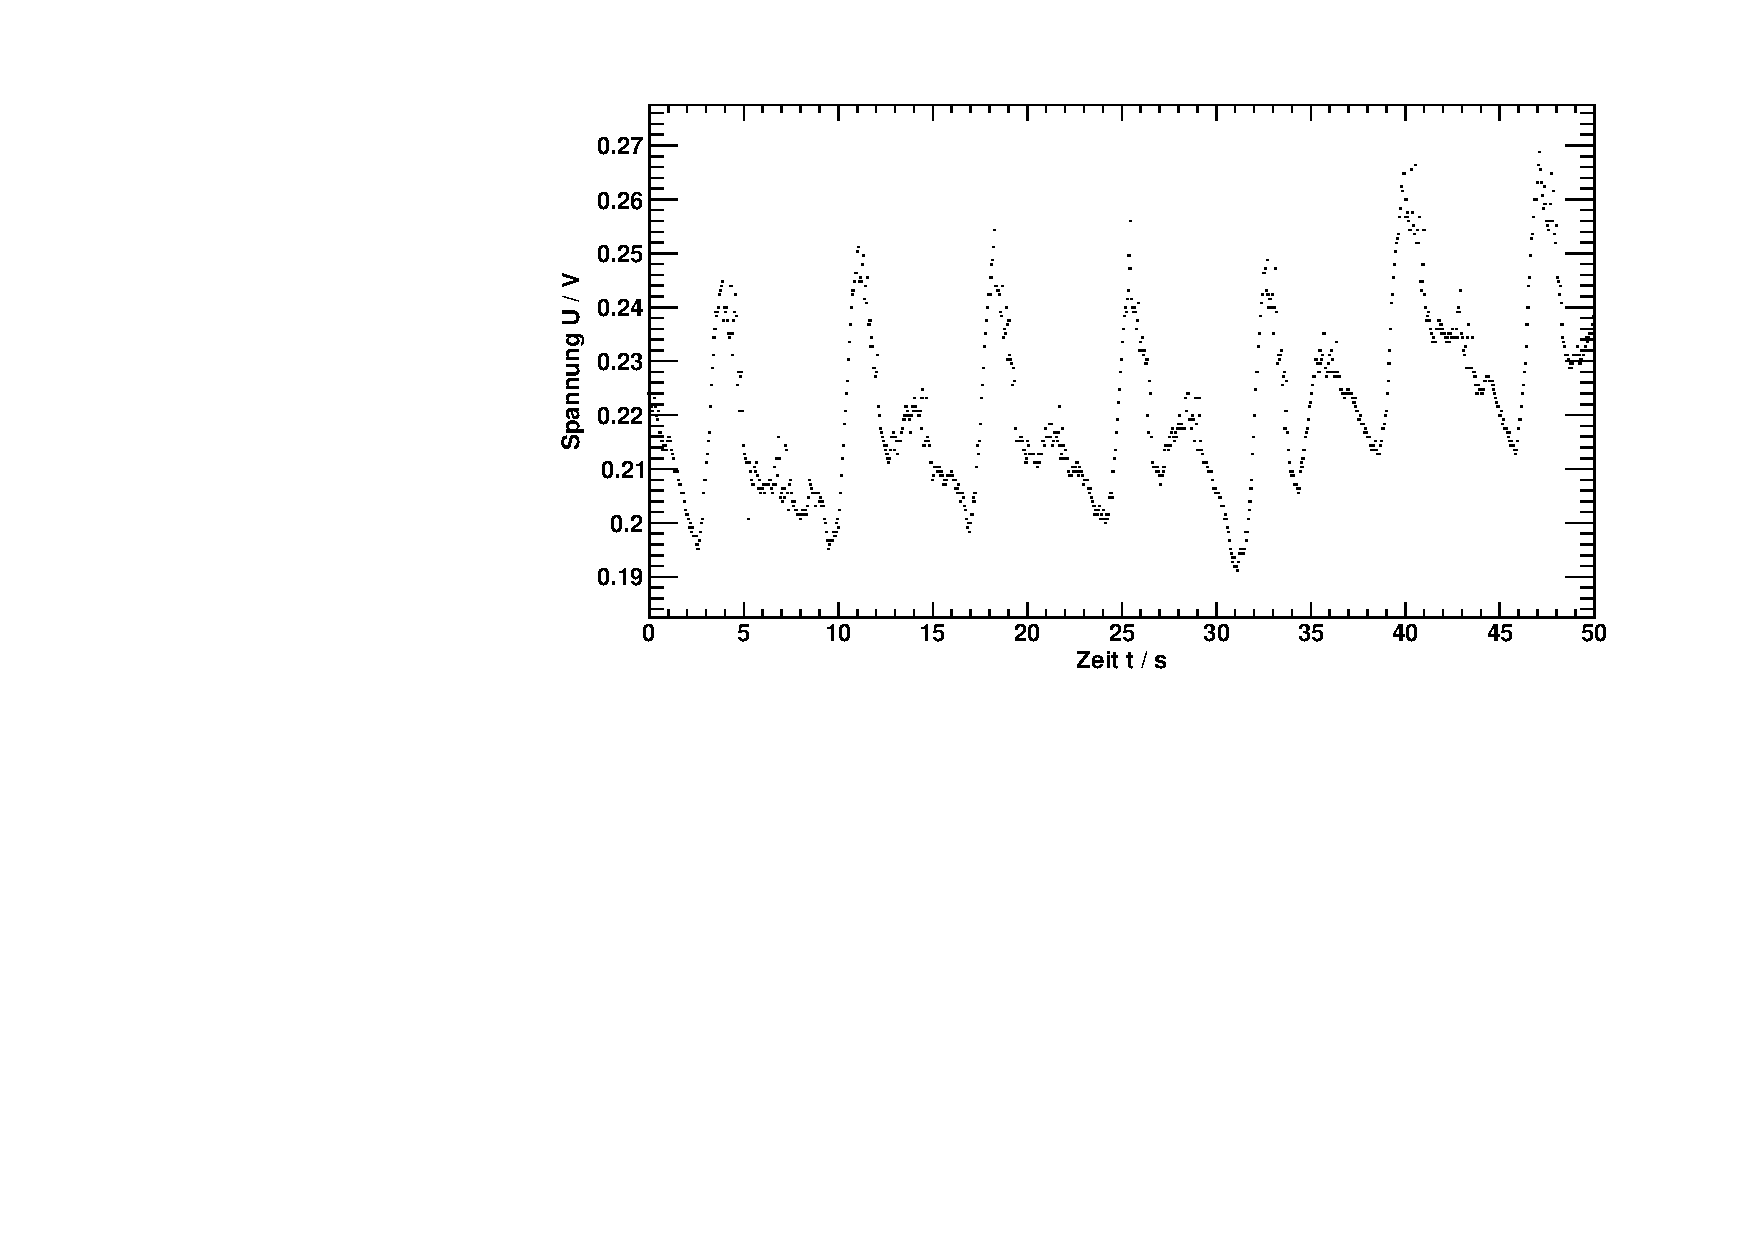
\includegraphics[width=0.64\textwidth]{../img/Au-Plaettchen.pdf}
  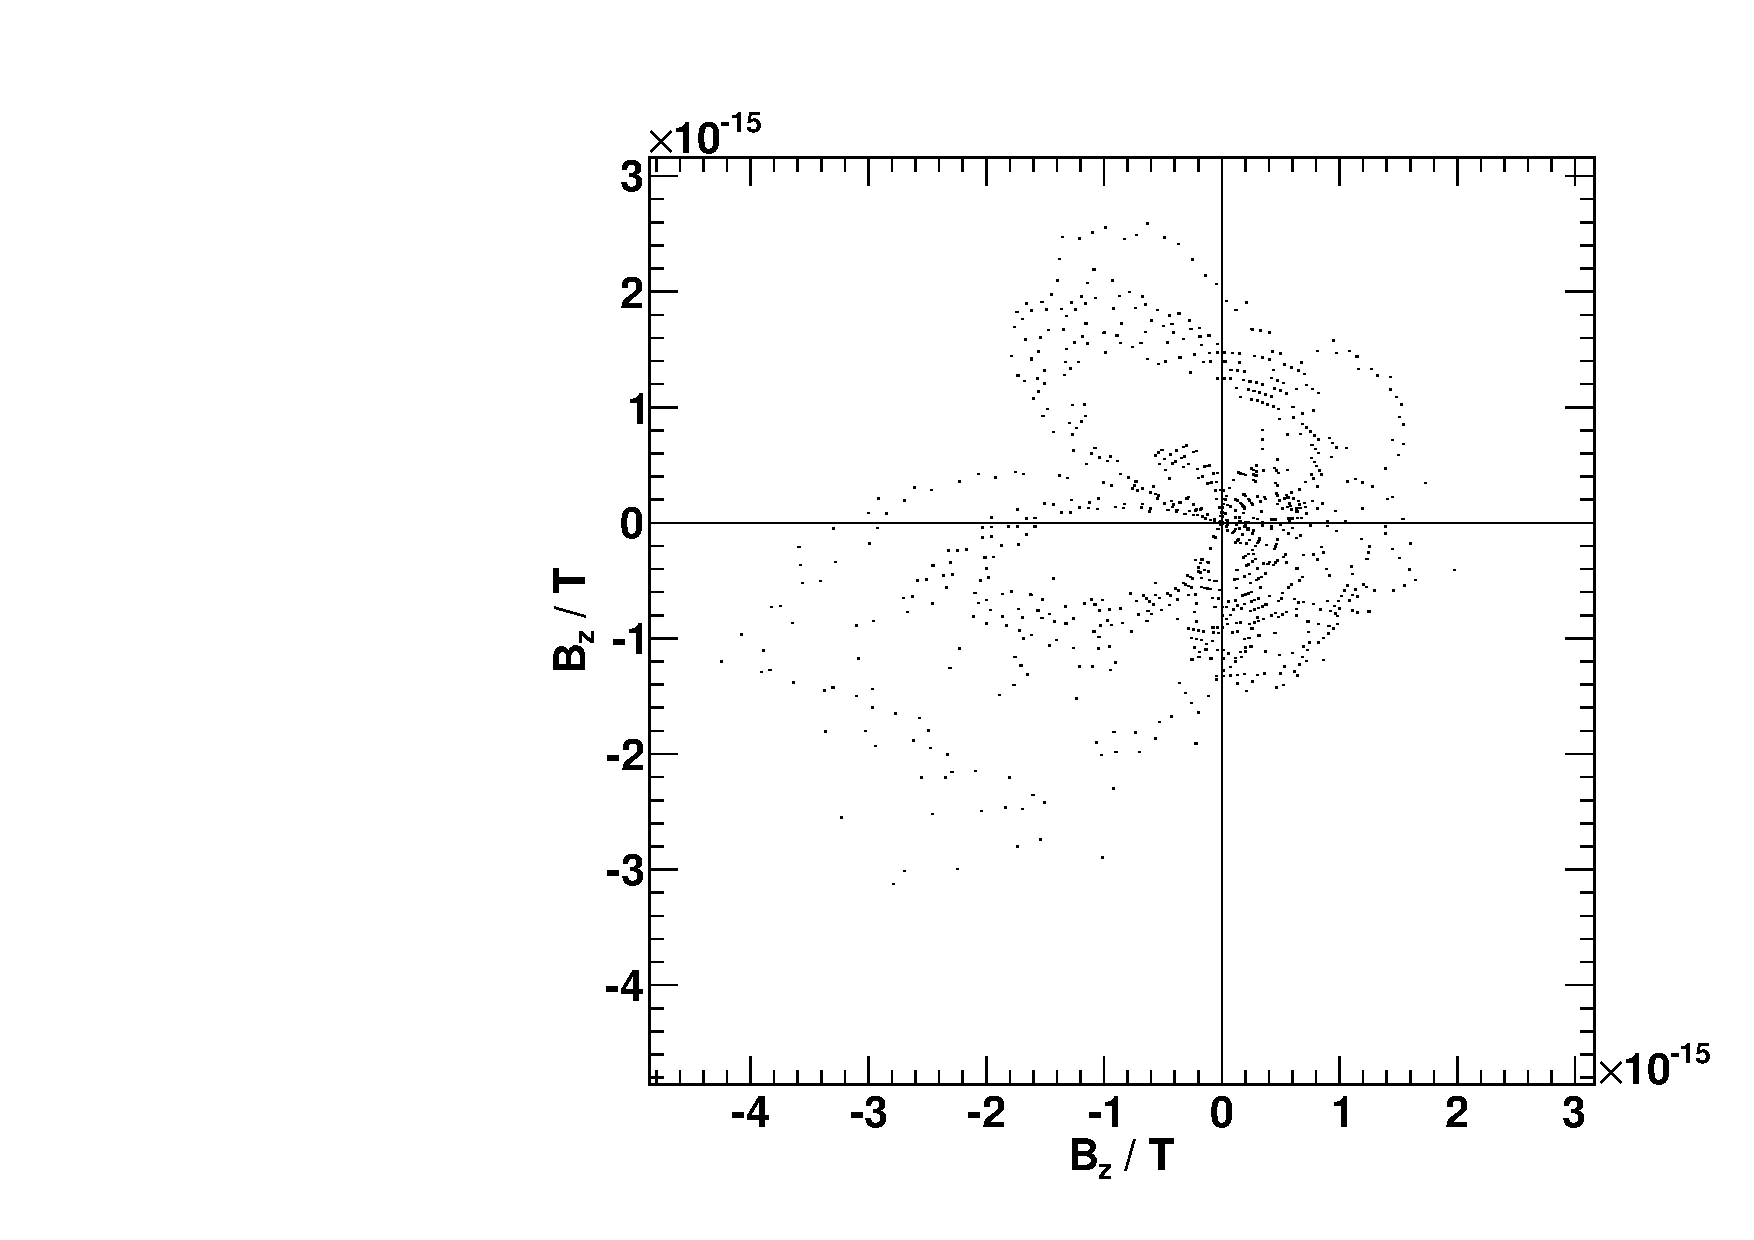
\includegraphics[width=0.35\textwidth]{../img/polar_Au-Plaettchen.pdf}
  \caption{Bestimmung des Magnetfelds eines Goldplättchens. Das periodische Signal stammt vermutlich
  vom magnetisierten Probenhalter (\autoref{img:holder}).}
  \label{img:au}
\end{center}
\end{figure}

Auch das Goldplättchen besitzt kein messbares Magnetfeld,
hier wird ebenfalls nur das Signal des Probenhalters gemessen.

